\begin{figure}[H] \centering % Created by tikzDevice version 0.12.4 on 2023-07-19 21:56:44
% !TEX encoding = UTF-8 Unicode
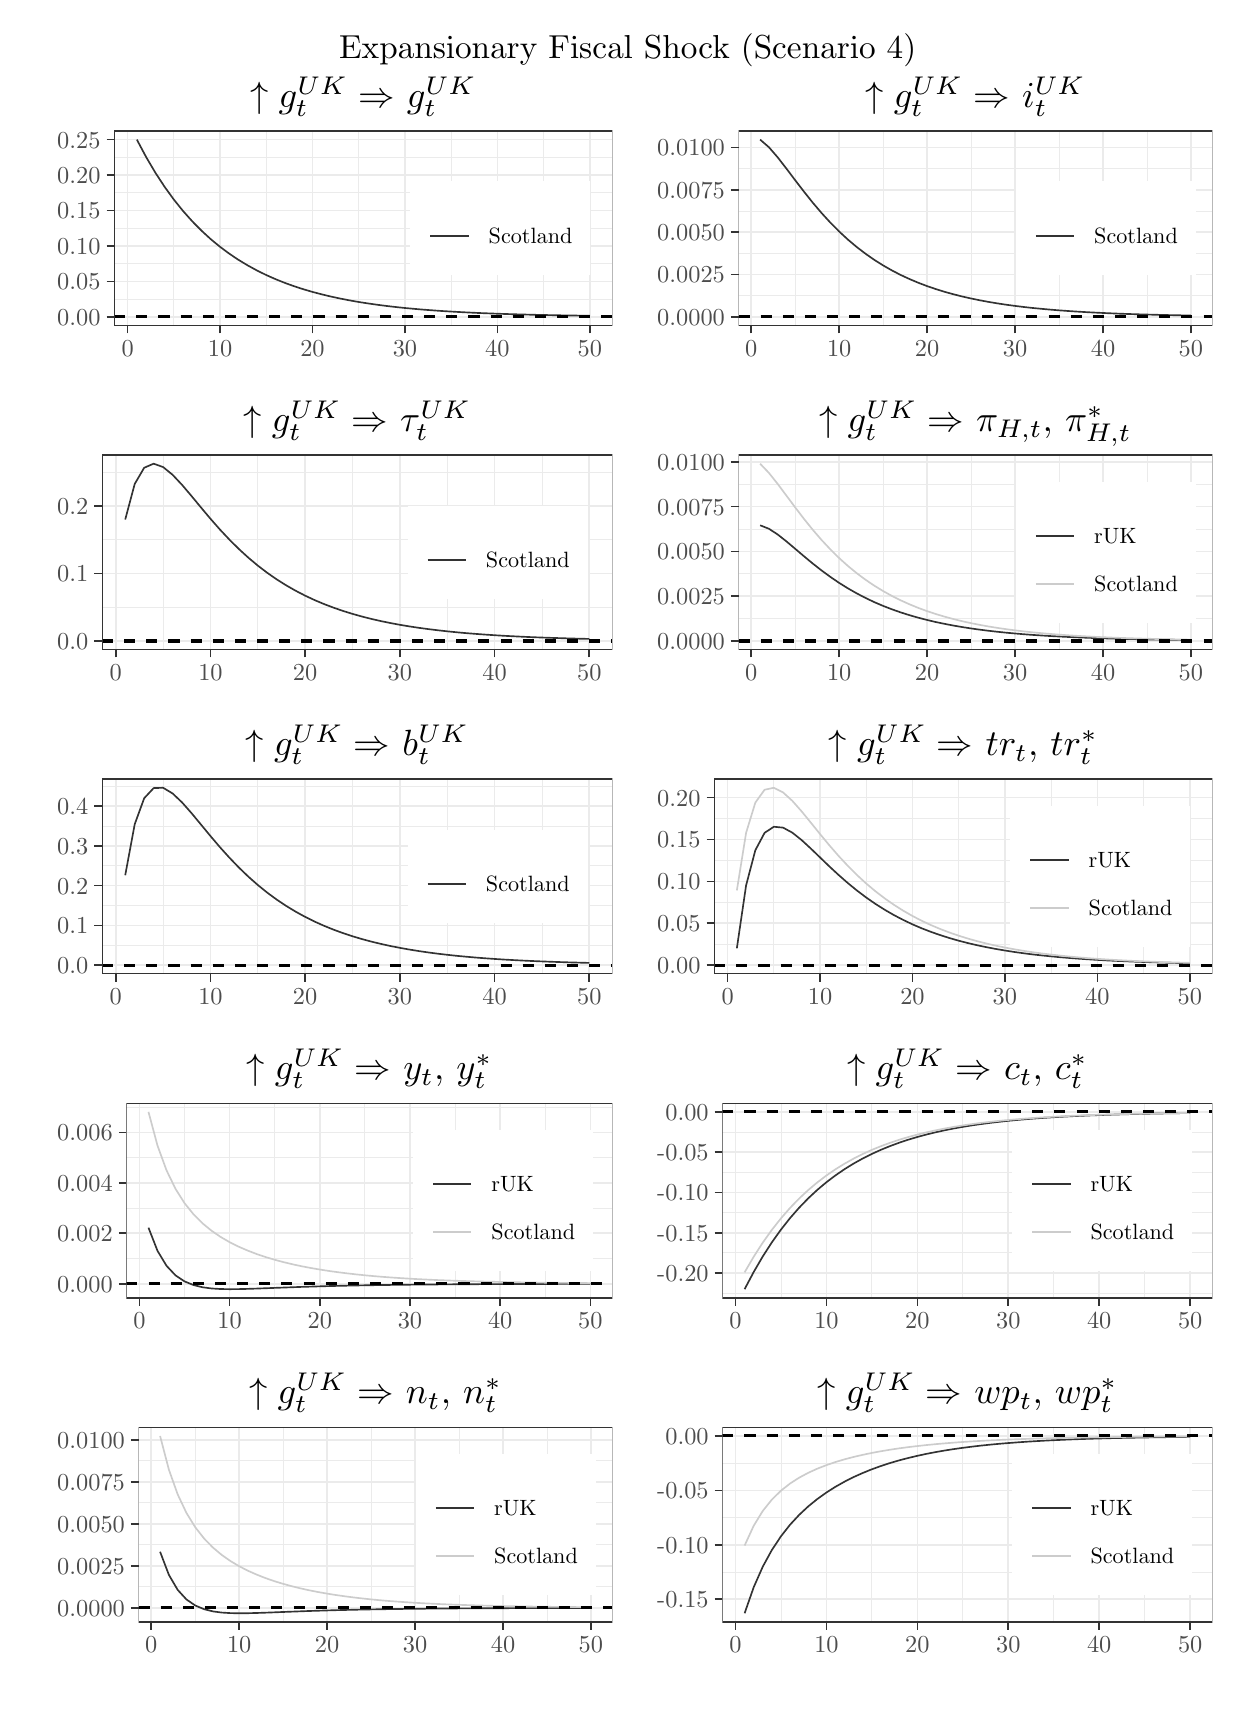
\begin{tikzpicture}[x=1pt,y=1pt]
\definecolor{fillColor}{RGB}{255,255,255}
\path[use as bounding box,fill=fillColor,fill opacity=0.00] (0,0) rectangle (433.62,599.84);
\begin{scope}
\path[clip] (  0.00,468.44) rectangle (216.81,585.55);
\definecolor{drawColor}{RGB}{255,255,255}
\definecolor{fillColor}{RGB}{255,255,255}

\path[draw=drawColor,line width= 0.6pt,line join=round,line cap=round,fill=fillColor] (  0.00,468.44) rectangle (216.81,585.55);
\end{scope}
\begin{scope}
\path[clip] ( 31.27,492.12) rectangle (211.31,562.59);
\definecolor{fillColor}{RGB}{255,255,255}

\path[fill=fillColor] ( 31.27,492.12) rectangle (211.31,562.59);
\definecolor{drawColor}{gray}{0.92}

\path[draw=drawColor,line width= 0.3pt,line join=round] ( 31.27,501.73) --
	(211.31,501.73);

\path[draw=drawColor,line width= 0.3pt,line join=round] ( 31.27,514.54) --
	(211.31,514.54);

\path[draw=drawColor,line width= 0.3pt,line join=round] ( 31.27,527.36) --
	(211.31,527.36);

\path[draw=drawColor,line width= 0.3pt,line join=round] ( 31.27,540.17) --
	(211.31,540.17);

\path[draw=drawColor,line width= 0.3pt,line join=round] ( 31.27,552.98) --
	(211.31,552.98);

\path[draw=drawColor,line width= 0.3pt,line join=round] ( 52.81,492.12) --
	( 52.81,562.59);

\path[draw=drawColor,line width= 0.3pt,line join=round] ( 86.22,492.12) --
	( 86.22,562.59);

\path[draw=drawColor,line width= 0.3pt,line join=round] (119.62,492.12) --
	(119.62,562.59);

\path[draw=drawColor,line width= 0.3pt,line join=round] (153.02,492.12) --
	(153.02,562.59);

\path[draw=drawColor,line width= 0.3pt,line join=round] (186.43,492.12) --
	(186.43,562.59);

\path[draw=drawColor,line width= 0.6pt,line join=round] ( 31.27,495.32) --
	(211.31,495.32);

\path[draw=drawColor,line width= 0.6pt,line join=round] ( 31.27,508.14) --
	(211.31,508.14);

\path[draw=drawColor,line width= 0.6pt,line join=round] ( 31.27,520.95) --
	(211.31,520.95);

\path[draw=drawColor,line width= 0.6pt,line join=round] ( 31.27,533.76) --
	(211.31,533.76);

\path[draw=drawColor,line width= 0.6pt,line join=round] ( 31.27,546.58) --
	(211.31,546.58);

\path[draw=drawColor,line width= 0.6pt,line join=round] ( 31.27,559.39) --
	(211.31,559.39);

\path[draw=drawColor,line width= 0.6pt,line join=round] ( 36.11,492.12) --
	( 36.11,562.59);

\path[draw=drawColor,line width= 0.6pt,line join=round] ( 69.52,492.12) --
	( 69.52,562.59);

\path[draw=drawColor,line width= 0.6pt,line join=round] (102.92,492.12) --
	(102.92,562.59);

\path[draw=drawColor,line width= 0.6pt,line join=round] (136.32,492.12) --
	(136.32,562.59);

\path[draw=drawColor,line width= 0.6pt,line join=round] (169.72,492.12) --
	(169.72,562.59);

\path[draw=drawColor,line width= 0.6pt,line join=round] (203.13,492.12) --
	(203.13,562.59);
\definecolor{drawColor}{gray}{0.20}

\path[draw=drawColor,line width= 0.6pt,line join=round] ( 39.45,559.39) --
	( 42.79,553.11) --
	( 46.13,547.45) --
	( 49.47,542.34) --
	( 52.81,537.73) --
	( 56.15,533.58) --
	( 59.50,529.83) --
	( 62.84,526.45) --
	( 66.18,523.39) --
	( 69.52,520.64) --
	( 72.86,518.16) --
	( 76.20,515.92) --
	( 79.54,513.91) --
	( 82.88,512.08) --
	( 86.22,510.44) --
	( 89.56,508.96) --
	( 92.90,507.62) --
	( 96.24,506.42) --
	( 99.58,505.33) --
	(102.92,504.35) --
	(106.26,503.47) --
	(109.60,502.67) --
	(112.94,501.95) --
	(116.28,501.30) --
	(119.62,500.71) --
	(122.96,500.19) --
	(126.30,499.71) --
	(129.64,499.28) --
	(132.98,498.89) --
	(136.32,498.54) --
	(139.66,498.23) --
	(143.00,497.94) --
	(146.34,497.69) --
	(149.68,497.45) --
	(153.02,497.25) --
	(156.36,497.06) --
	(159.70,496.89) --
	(163.04,496.73) --
	(166.38,496.60) --
	(169.72,496.47) --
	(173.06,496.36) --
	(176.40,496.26) --
	(179.74,496.17) --
	(183.08,496.08) --
	(186.43,496.01) --
	(189.77,495.94) --
	(193.11,495.88) --
	(196.45,495.83) --
	(199.79,495.78) --
	(203.13,495.73);
\definecolor{drawColor}{RGB}{0,0,0}

\path[draw=drawColor,line width= 1.1pt,dash pattern=on 4pt off 4pt ,line join=round] ( 31.27,495.32) -- (211.31,495.32);
\definecolor{drawColor}{gray}{0.20}

\path[draw=drawColor,line width= 0.6pt,line join=round,line cap=round] ( 31.27,492.12) rectangle (211.31,562.59);
\end{scope}
\begin{scope}
\path[clip] (  0.00,  0.00) rectangle (433.62,599.84);
\definecolor{drawColor}{gray}{0.30}

\node[text=drawColor,anchor=base east,inner sep=0pt, outer sep=0pt, scale=  0.88] at ( 26.32,492.29) {0.00};

\node[text=drawColor,anchor=base east,inner sep=0pt, outer sep=0pt, scale=  0.88] at ( 26.32,505.11) {0.05};

\node[text=drawColor,anchor=base east,inner sep=0pt, outer sep=0pt, scale=  0.88] at ( 26.32,517.92) {0.10};

\node[text=drawColor,anchor=base east,inner sep=0pt, outer sep=0pt, scale=  0.88] at ( 26.32,530.73) {0.15};

\node[text=drawColor,anchor=base east,inner sep=0pt, outer sep=0pt, scale=  0.88] at ( 26.32,543.55) {0.20};

\node[text=drawColor,anchor=base east,inner sep=0pt, outer sep=0pt, scale=  0.88] at ( 26.32,556.36) {0.25};
\end{scope}
\begin{scope}
\path[clip] (  0.00,  0.00) rectangle (433.62,599.84);
\definecolor{drawColor}{gray}{0.20}

\path[draw=drawColor,line width= 0.6pt,line join=round] ( 28.52,495.32) --
	( 31.27,495.32);

\path[draw=drawColor,line width= 0.6pt,line join=round] ( 28.52,508.14) --
	( 31.27,508.14);

\path[draw=drawColor,line width= 0.6pt,line join=round] ( 28.52,520.95) --
	( 31.27,520.95);

\path[draw=drawColor,line width= 0.6pt,line join=round] ( 28.52,533.76) --
	( 31.27,533.76);

\path[draw=drawColor,line width= 0.6pt,line join=round] ( 28.52,546.58) --
	( 31.27,546.58);

\path[draw=drawColor,line width= 0.6pt,line join=round] ( 28.52,559.39) --
	( 31.27,559.39);
\end{scope}
\begin{scope}
\path[clip] (  0.00,  0.00) rectangle (433.62,599.84);
\definecolor{drawColor}{gray}{0.20}

\path[draw=drawColor,line width= 0.6pt,line join=round] ( 36.11,489.37) --
	( 36.11,492.12);

\path[draw=drawColor,line width= 0.6pt,line join=round] ( 69.52,489.37) --
	( 69.52,492.12);

\path[draw=drawColor,line width= 0.6pt,line join=round] (102.92,489.37) --
	(102.92,492.12);

\path[draw=drawColor,line width= 0.6pt,line join=round] (136.32,489.37) --
	(136.32,492.12);

\path[draw=drawColor,line width= 0.6pt,line join=round] (169.72,489.37) --
	(169.72,492.12);

\path[draw=drawColor,line width= 0.6pt,line join=round] (203.13,489.37) --
	(203.13,492.12);
\end{scope}
\begin{scope}
\path[clip] (  0.00,  0.00) rectangle (433.62,599.84);
\definecolor{drawColor}{gray}{0.30}

\node[text=drawColor,anchor=base,inner sep=0pt, outer sep=0pt, scale=  0.88] at ( 36.11,481.11) {0};

\node[text=drawColor,anchor=base,inner sep=0pt, outer sep=0pt, scale=  0.88] at ( 69.52,481.11) {10};

\node[text=drawColor,anchor=base,inner sep=0pt, outer sep=0pt, scale=  0.88] at (102.92,481.11) {20};

\node[text=drawColor,anchor=base,inner sep=0pt, outer sep=0pt, scale=  0.88] at (136.32,481.11) {30};

\node[text=drawColor,anchor=base,inner sep=0pt, outer sep=0pt, scale=  0.88] at (169.72,481.11) {40};

\node[text=drawColor,anchor=base,inner sep=0pt, outer sep=0pt, scale=  0.88] at (203.13,481.11) {50};
\end{scope}
\begin{scope}
\path[clip] (  0.00,  0.00) rectangle (433.62,599.84);
\definecolor{fillColor}{RGB}{255,255,255}

\path[fill=fillColor] (138.26,510.43) rectangle (203.35,544.28);
\end{scope}
\begin{scope}
\path[clip] (  0.00,  0.00) rectangle (433.62,599.84);
\definecolor{fillColor}{RGB}{255,255,255}

\path[fill=fillColor] (143.76,515.93) rectangle (161.10,533.28);
\end{scope}
\begin{scope}
\path[clip] (  0.00,  0.00) rectangle (433.62,599.84);
\definecolor{drawColor}{gray}{0.20}

\path[draw=drawColor,line width= 0.6pt,line join=round] (145.49,524.61) -- (159.37,524.61);
\end{scope}
\begin{scope}
\path[clip] (  0.00,  0.00) rectangle (433.62,599.84);
\definecolor{drawColor}{RGB}{0,0,0}

\node[text=drawColor,anchor=base west,inner sep=0pt, outer sep=0pt, scale=  0.80] at (166.60,521.85) {Scotland};
\end{scope}
\begin{scope}
\path[clip] (  0.00,  0.00) rectangle (433.62,599.84);
\definecolor{drawColor}{RGB}{0,0,0}

\node[text=drawColor,anchor=base,inner sep=0pt, outer sep=0pt, scale=  1.32] at (121.29,570.96) {$\uparrow  g^{UK}_t \Rightarrow $ ${g^{UK}_t}$};
\end{scope}
\begin{scope}
\path[clip] (216.81,468.44) rectangle (433.62,585.55);
\definecolor{drawColor}{RGB}{255,255,255}
\definecolor{fillColor}{RGB}{255,255,255}

\path[draw=drawColor,line width= 0.6pt,line join=round,line cap=round,fill=fillColor] (216.81,468.44) rectangle (433.62,585.55);
\end{scope}
\begin{scope}
\path[clip] (256.88,492.12) rectangle (428.12,562.59);
\definecolor{fillColor}{RGB}{255,255,255}

\path[fill=fillColor] (256.88,492.12) rectangle (428.12,562.59);
\definecolor{drawColor}{gray}{0.92}

\path[draw=drawColor,line width= 0.3pt,line join=round] (256.88,502.98) --
	(428.12,502.98);

\path[draw=drawColor,line width= 0.3pt,line join=round] (256.88,518.29) --
	(428.12,518.29);

\path[draw=drawColor,line width= 0.3pt,line join=round] (256.88,533.61) --
	(428.12,533.61);

\path[draw=drawColor,line width= 0.3pt,line join=round] (256.88,548.92) --
	(428.12,548.92);

\path[draw=drawColor,line width= 0.3pt,line join=round] (277.37,492.12) --
	(277.37,562.59);

\path[draw=drawColor,line width= 0.3pt,line join=round] (309.14,492.12) --
	(309.14,562.59);

\path[draw=drawColor,line width= 0.3pt,line join=round] (340.91,492.12) --
	(340.91,562.59);

\path[draw=drawColor,line width= 0.3pt,line join=round] (372.68,492.12) --
	(372.68,562.59);

\path[draw=drawColor,line width= 0.3pt,line join=round] (404.45,492.12) --
	(404.45,562.59);

\path[draw=drawColor,line width= 0.6pt,line join=round] (256.88,495.32) --
	(428.12,495.32);

\path[draw=drawColor,line width= 0.6pt,line join=round] (256.88,510.64) --
	(428.12,510.64);

\path[draw=drawColor,line width= 0.6pt,line join=round] (256.88,525.95) --
	(428.12,525.95);

\path[draw=drawColor,line width= 0.6pt,line join=round] (256.88,541.26) --
	(428.12,541.26);

\path[draw=drawColor,line width= 0.6pt,line join=round] (256.88,556.58) --
	(428.12,556.58);

\path[draw=drawColor,line width= 0.6pt,line join=round] (261.48,492.12) --
	(261.48,562.59);

\path[draw=drawColor,line width= 0.6pt,line join=round] (293.25,492.12) --
	(293.25,562.59);

\path[draw=drawColor,line width= 0.6pt,line join=round] (325.03,492.12) --
	(325.03,562.59);

\path[draw=drawColor,line width= 0.6pt,line join=round] (356.80,492.12) --
	(356.80,562.59);

\path[draw=drawColor,line width= 0.6pt,line join=round] (388.57,492.12) --
	(388.57,562.59);

\path[draw=drawColor,line width= 0.6pt,line join=round] (420.34,492.12) --
	(420.34,562.59);
\definecolor{drawColor}{gray}{0.20}

\path[draw=drawColor,line width= 0.6pt,line join=round] (264.66,559.39) --
	(267.84,556.64) --
	(271.02,552.97) --
	(274.19,548.88) --
	(277.37,544.67) --
	(280.55,540.53) --
	(283.72,536.56) --
	(286.90,532.83) --
	(290.08,529.35) --
	(293.25,526.16) --
	(296.43,523.22) --
	(299.61,520.55) --
	(302.79,518.12) --
	(305.96,515.91) --
	(309.14,513.91) --
	(312.32,512.10) --
	(315.49,510.46) --
	(318.67,508.99) --
	(321.85,507.65) --
	(325.03,506.44) --
	(328.20,505.36) --
	(331.38,504.37) --
	(334.56,503.49) --
	(337.73,502.69) --
	(340.91,501.97) --
	(344.09,501.32) --
	(347.26,500.73) --
	(350.44,500.20) --
	(353.62,499.72) --
	(356.80,499.29) --
	(359.97,498.90) --
	(363.15,498.55) --
	(366.33,498.24) --
	(369.50,497.95) --
	(372.68,497.69) --
	(375.86,497.46) --
	(379.03,497.25) --
	(382.21,497.06) --
	(385.39,496.89) --
	(388.57,496.74) --
	(391.74,496.60) --
	(394.92,496.47) --
	(398.10,496.36) --
	(401.27,496.26) --
	(404.45,496.17) --
	(407.63,496.09) --
	(410.81,496.01) --
	(413.98,495.94) --
	(417.16,495.88) --
	(420.34,495.83);
\definecolor{drawColor}{RGB}{0,0,0}

\path[draw=drawColor,line width= 1.1pt,dash pattern=on 4pt off 4pt ,line join=round] (256.88,495.32) -- (428.12,495.32);
\definecolor{drawColor}{gray}{0.20}

\path[draw=drawColor,line width= 0.6pt,line join=round,line cap=round] (256.88,492.12) rectangle (428.12,562.59);
\end{scope}
\begin{scope}
\path[clip] (  0.00,  0.00) rectangle (433.62,599.84);
\definecolor{drawColor}{gray}{0.30}

\node[text=drawColor,anchor=base east,inner sep=0pt, outer sep=0pt, scale=  0.88] at (251.93,492.29) {0.0000};

\node[text=drawColor,anchor=base east,inner sep=0pt, outer sep=0pt, scale=  0.88] at (251.93,507.61) {0.0025};

\node[text=drawColor,anchor=base east,inner sep=0pt, outer sep=0pt, scale=  0.88] at (251.93,522.92) {0.0050};

\node[text=drawColor,anchor=base east,inner sep=0pt, outer sep=0pt, scale=  0.88] at (251.93,538.23) {0.0075};

\node[text=drawColor,anchor=base east,inner sep=0pt, outer sep=0pt, scale=  0.88] at (251.93,553.55) {0.0100};
\end{scope}
\begin{scope}
\path[clip] (  0.00,  0.00) rectangle (433.62,599.84);
\definecolor{drawColor}{gray}{0.20}

\path[draw=drawColor,line width= 0.6pt,line join=round] (254.13,495.32) --
	(256.88,495.32);

\path[draw=drawColor,line width= 0.6pt,line join=round] (254.13,510.64) --
	(256.88,510.64);

\path[draw=drawColor,line width= 0.6pt,line join=round] (254.13,525.95) --
	(256.88,525.95);

\path[draw=drawColor,line width= 0.6pt,line join=round] (254.13,541.26) --
	(256.88,541.26);

\path[draw=drawColor,line width= 0.6pt,line join=round] (254.13,556.58) --
	(256.88,556.58);
\end{scope}
\begin{scope}
\path[clip] (  0.00,  0.00) rectangle (433.62,599.84);
\definecolor{drawColor}{gray}{0.20}

\path[draw=drawColor,line width= 0.6pt,line join=round] (261.48,489.37) --
	(261.48,492.12);

\path[draw=drawColor,line width= 0.6pt,line join=round] (293.25,489.37) --
	(293.25,492.12);

\path[draw=drawColor,line width= 0.6pt,line join=round] (325.03,489.37) --
	(325.03,492.12);

\path[draw=drawColor,line width= 0.6pt,line join=round] (356.80,489.37) --
	(356.80,492.12);

\path[draw=drawColor,line width= 0.6pt,line join=round] (388.57,489.37) --
	(388.57,492.12);

\path[draw=drawColor,line width= 0.6pt,line join=round] (420.34,489.37) --
	(420.34,492.12);
\end{scope}
\begin{scope}
\path[clip] (  0.00,  0.00) rectangle (433.62,599.84);
\definecolor{drawColor}{gray}{0.30}

\node[text=drawColor,anchor=base,inner sep=0pt, outer sep=0pt, scale=  0.88] at (261.48,481.11) {0};

\node[text=drawColor,anchor=base,inner sep=0pt, outer sep=0pt, scale=  0.88] at (293.25,481.11) {10};

\node[text=drawColor,anchor=base,inner sep=0pt, outer sep=0pt, scale=  0.88] at (325.03,481.11) {20};

\node[text=drawColor,anchor=base,inner sep=0pt, outer sep=0pt, scale=  0.88] at (356.80,481.11) {30};

\node[text=drawColor,anchor=base,inner sep=0pt, outer sep=0pt, scale=  0.88] at (388.57,481.11) {40};

\node[text=drawColor,anchor=base,inner sep=0pt, outer sep=0pt, scale=  0.88] at (420.34,481.11) {50};
\end{scope}
\begin{scope}
\path[clip] (  0.00,  0.00) rectangle (433.62,599.84);
\definecolor{fillColor}{RGB}{255,255,255}

\path[fill=fillColor] (357.05,510.43) rectangle (422.14,544.28);
\end{scope}
\begin{scope}
\path[clip] (  0.00,  0.00) rectangle (433.62,599.84);
\definecolor{fillColor}{RGB}{255,255,255}

\path[fill=fillColor] (362.55,515.93) rectangle (379.89,533.28);
\end{scope}
\begin{scope}
\path[clip] (  0.00,  0.00) rectangle (433.62,599.84);
\definecolor{drawColor}{gray}{0.20}

\path[draw=drawColor,line width= 0.6pt,line join=round] (364.28,524.61) -- (378.16,524.61);
\end{scope}
\begin{scope}
\path[clip] (  0.00,  0.00) rectangle (433.62,599.84);
\definecolor{drawColor}{RGB}{0,0,0}

\node[text=drawColor,anchor=base west,inner sep=0pt, outer sep=0pt, scale=  0.80] at (385.39,521.85) {Scotland};
\end{scope}
\begin{scope}
\path[clip] (  0.00,  0.00) rectangle (433.62,599.84);
\definecolor{drawColor}{RGB}{0,0,0}

\node[text=drawColor,anchor=base,inner sep=0pt, outer sep=0pt, scale=  1.32] at (342.50,570.96) {$\uparrow  g^{UK}_t \Rightarrow $ ${i^{UK}_t}$};
\end{scope}
\begin{scope}
\path[clip] (  0.00,351.33) rectangle (216.81,468.44);
\definecolor{drawColor}{RGB}{255,255,255}
\definecolor{fillColor}{RGB}{255,255,255}

\path[draw=drawColor,line width= 0.6pt,line join=round,line cap=round,fill=fillColor] (  0.00,351.33) rectangle (216.81,468.44);
\end{scope}
\begin{scope}
\path[clip] ( 26.87,375.01) rectangle (211.31,445.48);
\definecolor{fillColor}{RGB}{255,255,255}

\path[fill=fillColor] ( 26.87,375.01) rectangle (211.31,445.48);
\definecolor{drawColor}{gray}{0.92}

\path[draw=drawColor,line width= 0.3pt,line join=round] ( 26.87,390.43) --
	(211.31,390.43);

\path[draw=drawColor,line width= 0.3pt,line join=round] ( 26.87,414.87) --
	(211.31,414.87);

\path[draw=drawColor,line width= 0.3pt,line join=round] ( 26.87,439.30) --
	(211.31,439.30);

\path[draw=drawColor,line width= 0.3pt,line join=round] ( 48.94,375.01) --
	( 48.94,445.48);

\path[draw=drawColor,line width= 0.3pt,line join=round] ( 83.16,375.01) --
	( 83.16,445.48);

\path[draw=drawColor,line width= 0.3pt,line join=round] (117.38,375.01) --
	(117.38,445.48);

\path[draw=drawColor,line width= 0.3pt,line join=round] (151.60,375.01) --
	(151.60,445.48);

\path[draw=drawColor,line width= 0.3pt,line join=round] (185.82,375.01) --
	(185.82,445.48);

\path[draw=drawColor,line width= 0.6pt,line join=round] ( 26.87,378.21) --
	(211.31,378.21);

\path[draw=drawColor,line width= 0.6pt,line join=round] ( 26.87,402.65) --
	(211.31,402.65);

\path[draw=drawColor,line width= 0.6pt,line join=round] ( 26.87,427.09) --
	(211.31,427.09);

\path[draw=drawColor,line width= 0.6pt,line join=round] ( 31.83,375.01) --
	( 31.83,445.48);

\path[draw=drawColor,line width= 0.6pt,line join=round] ( 66.05,375.01) --
	( 66.05,445.48);

\path[draw=drawColor,line width= 0.6pt,line join=round] (100.27,375.01) --
	(100.27,445.48);

\path[draw=drawColor,line width= 0.6pt,line join=round] (134.49,375.01) --
	(134.49,445.48);

\path[draw=drawColor,line width= 0.6pt,line join=round] (168.71,375.01) --
	(168.71,445.48);

\path[draw=drawColor,line width= 0.6pt,line join=round] (202.93,375.01) --
	(202.93,445.48);
\definecolor{drawColor}{gray}{0.20}

\path[draw=drawColor,line width= 0.6pt,line join=round] ( 35.25,422.11) --
	( 38.68,434.96) --
	( 42.10,440.81) --
	( 45.52,442.28) --
	( 48.94,441.06) --
	( 52.36,438.27) --
	( 55.79,434.62) --
	( 59.21,430.59) --
	( 62.63,426.45) --
	( 66.05,422.38) --
	( 69.47,418.49) --
	( 72.90,414.84) --
	( 76.32,411.44) --
	( 79.74,408.32) --
	( 83.16,405.45) --
	( 86.58,402.84) --
	( 90.00,400.47) --
	( 93.43,398.31) --
	( 96.85,396.36) --
	(100.27,394.59) --
	(103.69,392.99) --
	(107.11,391.55) --
	(110.54,390.25) --
	(113.96,389.07) --
	(117.38,388.01) --
	(120.80,387.05) --
	(124.22,386.18) --
	(127.65,385.40) --
	(131.07,384.70) --
	(134.49,384.06) --
	(137.91,383.49) --
	(141.33,382.97) --
	(144.75,382.51) --
	(148.18,382.09) --
	(151.60,381.71) --
	(155.02,381.36) --
	(158.44,381.05) --
	(161.86,380.78) --
	(165.29,380.53) --
	(168.71,380.30) --
	(172.13,380.09) --
	(175.55,379.91) --
	(178.97,379.74) --
	(182.40,379.59) --
	(185.82,379.46) --
	(189.24,379.34) --
	(192.66,379.23) --
	(196.08,379.13) --
	(199.50,379.04) --
	(202.93,378.96);
\definecolor{drawColor}{RGB}{0,0,0}

\path[draw=drawColor,line width= 1.1pt,dash pattern=on 4pt off 4pt ,line join=round] ( 26.87,378.21) -- (211.31,378.21);
\definecolor{drawColor}{gray}{0.20}

\path[draw=drawColor,line width= 0.6pt,line join=round,line cap=round] ( 26.87,375.01) rectangle (211.31,445.48);
\end{scope}
\begin{scope}
\path[clip] (  0.00,  0.00) rectangle (433.62,599.84);
\definecolor{drawColor}{gray}{0.30}

\node[text=drawColor,anchor=base east,inner sep=0pt, outer sep=0pt, scale=  0.88] at ( 21.92,375.18) {0.0};

\node[text=drawColor,anchor=base east,inner sep=0pt, outer sep=0pt, scale=  0.88] at ( 21.92,399.62) {0.1};

\node[text=drawColor,anchor=base east,inner sep=0pt, outer sep=0pt, scale=  0.88] at ( 21.92,424.06) {0.2};
\end{scope}
\begin{scope}
\path[clip] (  0.00,  0.00) rectangle (433.62,599.84);
\definecolor{drawColor}{gray}{0.20}

\path[draw=drawColor,line width= 0.6pt,line join=round] ( 24.12,378.21) --
	( 26.87,378.21);

\path[draw=drawColor,line width= 0.6pt,line join=round] ( 24.12,402.65) --
	( 26.87,402.65);

\path[draw=drawColor,line width= 0.6pt,line join=round] ( 24.12,427.09) --
	( 26.87,427.09);
\end{scope}
\begin{scope}
\path[clip] (  0.00,  0.00) rectangle (433.62,599.84);
\definecolor{drawColor}{gray}{0.20}

\path[draw=drawColor,line width= 0.6pt,line join=round] ( 31.83,372.26) --
	( 31.83,375.01);

\path[draw=drawColor,line width= 0.6pt,line join=round] ( 66.05,372.26) --
	( 66.05,375.01);

\path[draw=drawColor,line width= 0.6pt,line join=round] (100.27,372.26) --
	(100.27,375.01);

\path[draw=drawColor,line width= 0.6pt,line join=round] (134.49,372.26) --
	(134.49,375.01);

\path[draw=drawColor,line width= 0.6pt,line join=round] (168.71,372.26) --
	(168.71,375.01);

\path[draw=drawColor,line width= 0.6pt,line join=round] (202.93,372.26) --
	(202.93,375.01);
\end{scope}
\begin{scope}
\path[clip] (  0.00,  0.00) rectangle (433.62,599.84);
\definecolor{drawColor}{gray}{0.30}

\node[text=drawColor,anchor=base,inner sep=0pt, outer sep=0pt, scale=  0.88] at ( 31.83,364.00) {0};

\node[text=drawColor,anchor=base,inner sep=0pt, outer sep=0pt, scale=  0.88] at ( 66.05,364.00) {10};

\node[text=drawColor,anchor=base,inner sep=0pt, outer sep=0pt, scale=  0.88] at (100.27,364.00) {20};

\node[text=drawColor,anchor=base,inner sep=0pt, outer sep=0pt, scale=  0.88] at (134.49,364.00) {30};

\node[text=drawColor,anchor=base,inner sep=0pt, outer sep=0pt, scale=  0.88] at (168.71,364.00) {40};

\node[text=drawColor,anchor=base,inner sep=0pt, outer sep=0pt, scale=  0.88] at (202.93,364.00) {50};
\end{scope}
\begin{scope}
\path[clip] (  0.00,  0.00) rectangle (433.62,599.84);
\definecolor{fillColor}{RGB}{255,255,255}

\path[fill=fillColor] (137.27,393.32) rectangle (202.36,427.17);
\end{scope}
\begin{scope}
\path[clip] (  0.00,  0.00) rectangle (433.62,599.84);
\definecolor{fillColor}{RGB}{255,255,255}

\path[fill=fillColor] (142.77,398.82) rectangle (160.11,416.17);
\end{scope}
\begin{scope}
\path[clip] (  0.00,  0.00) rectangle (433.62,599.84);
\definecolor{drawColor}{gray}{0.20}

\path[draw=drawColor,line width= 0.6pt,line join=round] (144.50,407.50) -- (158.38,407.50);
\end{scope}
\begin{scope}
\path[clip] (  0.00,  0.00) rectangle (433.62,599.84);
\definecolor{drawColor}{RGB}{0,0,0}

\node[text=drawColor,anchor=base west,inner sep=0pt, outer sep=0pt, scale=  0.80] at (165.61,404.74) {Scotland};
\end{scope}
\begin{scope}
\path[clip] (  0.00,  0.00) rectangle (433.62,599.84);
\definecolor{drawColor}{RGB}{0,0,0}

\node[text=drawColor,anchor=base,inner sep=0pt, outer sep=0pt, scale=  1.32] at (119.09,453.85) {$\uparrow  g^{UK}_t \Rightarrow $ ${\tau^{UK}_t}$};
\end{scope}
\begin{scope}
\path[clip] (216.81,351.33) rectangle (433.62,468.44);
\definecolor{drawColor}{RGB}{255,255,255}
\definecolor{fillColor}{RGB}{255,255,255}

\path[draw=drawColor,line width= 0.6pt,line join=round,line cap=round,fill=fillColor] (216.81,351.33) rectangle (433.62,468.44);
\end{scope}
\begin{scope}
\path[clip] (256.88,375.01) rectangle (428.12,445.48);
\definecolor{fillColor}{RGB}{255,255,255}

\path[fill=fillColor] (256.88,375.01) rectangle (428.12,445.48);
\definecolor{drawColor}{gray}{0.92}

\path[draw=drawColor,line width= 0.3pt,line join=round] (256.88,386.30) --
	(428.12,386.30);

\path[draw=drawColor,line width= 0.3pt,line join=round] (256.88,402.49) --
	(428.12,402.49);

\path[draw=drawColor,line width= 0.3pt,line join=round] (256.88,418.67) --
	(428.12,418.67);

\path[draw=drawColor,line width= 0.3pt,line join=round] (256.88,434.86) --
	(428.12,434.86);

\path[draw=drawColor,line width= 0.3pt,line join=round] (277.37,375.01) --
	(277.37,445.48);

\path[draw=drawColor,line width= 0.3pt,line join=round] (309.14,375.01) --
	(309.14,445.48);

\path[draw=drawColor,line width= 0.3pt,line join=round] (340.91,375.01) --
	(340.91,445.48);

\path[draw=drawColor,line width= 0.3pt,line join=round] (372.68,375.01) --
	(372.68,445.48);

\path[draw=drawColor,line width= 0.3pt,line join=round] (404.45,375.01) --
	(404.45,445.48);

\path[draw=drawColor,line width= 0.6pt,line join=round] (256.88,378.21) --
	(428.12,378.21);

\path[draw=drawColor,line width= 0.6pt,line join=round] (256.88,394.40) --
	(428.12,394.40);

\path[draw=drawColor,line width= 0.6pt,line join=round] (256.88,410.58) --
	(428.12,410.58);

\path[draw=drawColor,line width= 0.6pt,line join=round] (256.88,426.77) --
	(428.12,426.77);

\path[draw=drawColor,line width= 0.6pt,line join=round] (256.88,442.95) --
	(428.12,442.95);

\path[draw=drawColor,line width= 0.6pt,line join=round] (261.48,375.01) --
	(261.48,445.48);

\path[draw=drawColor,line width= 0.6pt,line join=round] (293.25,375.01) --
	(293.25,445.48);

\path[draw=drawColor,line width= 0.6pt,line join=round] (325.03,375.01) --
	(325.03,445.48);

\path[draw=drawColor,line width= 0.6pt,line join=round] (356.80,375.01) --
	(356.80,445.48);

\path[draw=drawColor,line width= 0.6pt,line join=round] (388.57,375.01) --
	(388.57,445.48);

\path[draw=drawColor,line width= 0.6pt,line join=round] (420.34,375.01) --
	(420.34,445.48);
\definecolor{drawColor}{gray}{0.20}

\path[draw=drawColor,line width= 0.6pt,line join=round] (264.66,420.02) --
	(267.84,418.77) --
	(271.02,416.69) --
	(274.19,414.19) --
	(277.37,411.50) --
	(280.55,408.80) --
	(283.72,406.17) --
	(286.90,403.68) --
	(290.08,401.35) --
	(293.25,399.19) --
	(296.43,397.21) --
	(299.61,395.40) --
	(302.79,393.75) --
	(305.96,392.24) --
	(309.14,390.88) --
	(312.32,389.65) --
	(315.49,388.54) --
	(318.67,387.53) --
	(321.85,386.62) --
	(325.03,385.80) --
	(328.20,385.05) --
	(331.38,384.39) --
	(334.56,383.78) --
	(337.73,383.24) --
	(340.91,382.74) --
	(344.09,382.30) --
	(347.26,381.90) --
	(350.44,381.54) --
	(353.62,381.21) --
	(356.80,380.92) --
	(359.97,380.65) --
	(363.15,380.41) --
	(366.33,380.20) --
	(369.50,380.00) --
	(372.68,379.83) --
	(375.86,379.67) --
	(379.03,379.53) --
	(382.21,379.40) --
	(385.39,379.28) --
	(388.57,379.18) --
	(391.74,379.08) --
	(394.92,379.00) --
	(398.10,378.92) --
	(401.27,378.85) --
	(404.45,378.79) --
	(407.63,378.73) --
	(410.81,378.68) --
	(413.98,378.64) --
	(417.16,378.59) --
	(420.34,378.56);
\definecolor{drawColor}{gray}{0.80}

\path[draw=drawColor,line width= 0.6pt,line join=round] (264.66,442.28) --
	(267.84,438.95) --
	(271.02,434.96) --
	(274.19,430.71) --
	(277.37,426.44) --
	(280.55,422.29) --
	(283.72,418.36) --
	(286.90,414.68) --
	(290.08,411.28) --
	(293.25,408.15) --
	(296.43,405.29) --
	(299.61,402.69) --
	(302.79,400.32) --
	(305.96,398.18) --
	(309.14,396.24) --
	(312.32,394.48) --
	(315.49,392.89) --
	(318.67,391.46) --
	(321.85,390.16) --
	(325.03,388.99) --
	(328.20,387.94) --
	(331.38,386.99) --
	(334.56,386.13) --
	(337.73,385.35) --
	(340.91,384.65) --
	(344.09,384.02) --
	(347.26,383.45) --
	(350.44,382.94) --
	(353.62,382.48) --
	(356.80,382.06) --
	(359.97,381.68) --
	(363.15,381.34) --
	(366.33,381.04) --
	(369.50,380.76) --
	(372.68,380.51) --
	(375.86,380.28) --
	(379.03,380.08) --
	(382.21,379.90) --
	(385.39,379.73) --
	(388.57,379.58) --
	(391.74,379.45) --
	(394.92,379.33) --
	(398.10,379.22) --
	(401.27,379.12) --
	(404.45,379.03) --
	(407.63,378.95) --
	(410.81,378.88) --
	(413.98,378.81) --
	(417.16,378.75) --
	(420.34,378.70);
\definecolor{drawColor}{RGB}{0,0,0}

\path[draw=drawColor,line width= 1.1pt,dash pattern=on 4pt off 4pt ,line join=round] (256.88,378.21) -- (428.12,378.21);
\definecolor{drawColor}{gray}{0.20}

\path[draw=drawColor,line width= 0.6pt,line join=round,line cap=round] (256.88,375.01) rectangle (428.12,445.48);
\end{scope}
\begin{scope}
\path[clip] (  0.00,  0.00) rectangle (433.62,599.84);
\definecolor{drawColor}{gray}{0.30}

\node[text=drawColor,anchor=base east,inner sep=0pt, outer sep=0pt, scale=  0.88] at (251.93,375.18) {0.0000};

\node[text=drawColor,anchor=base east,inner sep=0pt, outer sep=0pt, scale=  0.88] at (251.93,391.37) {0.0025};

\node[text=drawColor,anchor=base east,inner sep=0pt, outer sep=0pt, scale=  0.88] at (251.93,407.55) {0.0050};

\node[text=drawColor,anchor=base east,inner sep=0pt, outer sep=0pt, scale=  0.88] at (251.93,423.74) {0.0075};

\node[text=drawColor,anchor=base east,inner sep=0pt, outer sep=0pt, scale=  0.88] at (251.93,439.92) {0.0100};
\end{scope}
\begin{scope}
\path[clip] (  0.00,  0.00) rectangle (433.62,599.84);
\definecolor{drawColor}{gray}{0.20}

\path[draw=drawColor,line width= 0.6pt,line join=round] (254.13,378.21) --
	(256.88,378.21);

\path[draw=drawColor,line width= 0.6pt,line join=round] (254.13,394.40) --
	(256.88,394.40);

\path[draw=drawColor,line width= 0.6pt,line join=round] (254.13,410.58) --
	(256.88,410.58);

\path[draw=drawColor,line width= 0.6pt,line join=round] (254.13,426.77) --
	(256.88,426.77);

\path[draw=drawColor,line width= 0.6pt,line join=round] (254.13,442.95) --
	(256.88,442.95);
\end{scope}
\begin{scope}
\path[clip] (  0.00,  0.00) rectangle (433.62,599.84);
\definecolor{drawColor}{gray}{0.20}

\path[draw=drawColor,line width= 0.6pt,line join=round] (261.48,372.26) --
	(261.48,375.01);

\path[draw=drawColor,line width= 0.6pt,line join=round] (293.25,372.26) --
	(293.25,375.01);

\path[draw=drawColor,line width= 0.6pt,line join=round] (325.03,372.26) --
	(325.03,375.01);

\path[draw=drawColor,line width= 0.6pt,line join=round] (356.80,372.26) --
	(356.80,375.01);

\path[draw=drawColor,line width= 0.6pt,line join=round] (388.57,372.26) --
	(388.57,375.01);

\path[draw=drawColor,line width= 0.6pt,line join=round] (420.34,372.26) --
	(420.34,375.01);
\end{scope}
\begin{scope}
\path[clip] (  0.00,  0.00) rectangle (433.62,599.84);
\definecolor{drawColor}{gray}{0.30}

\node[text=drawColor,anchor=base,inner sep=0pt, outer sep=0pt, scale=  0.88] at (261.48,364.00) {0};

\node[text=drawColor,anchor=base,inner sep=0pt, outer sep=0pt, scale=  0.88] at (293.25,364.00) {10};

\node[text=drawColor,anchor=base,inner sep=0pt, outer sep=0pt, scale=  0.88] at (325.03,364.00) {20};

\node[text=drawColor,anchor=base,inner sep=0pt, outer sep=0pt, scale=  0.88] at (356.80,364.00) {30};

\node[text=drawColor,anchor=base,inner sep=0pt, outer sep=0pt, scale=  0.88] at (388.57,364.00) {40};

\node[text=drawColor,anchor=base,inner sep=0pt, outer sep=0pt, scale=  0.88] at (420.34,364.00) {50};
\end{scope}
\begin{scope}
\path[clip] (  0.00,  0.00) rectangle (433.62,599.84);
\definecolor{fillColor}{RGB}{255,255,255}

\path[fill=fillColor] (357.05,384.65) rectangle (422.14,435.84);
\end{scope}
\begin{scope}
\path[clip] (  0.00,  0.00) rectangle (433.62,599.84);
\definecolor{fillColor}{RGB}{255,255,255}

\path[fill=fillColor] (362.55,407.50) rectangle (379.89,424.84);
\end{scope}
\begin{scope}
\path[clip] (  0.00,  0.00) rectangle (433.62,599.84);
\definecolor{drawColor}{gray}{0.20}

\path[draw=drawColor,line width= 0.6pt,line join=round] (364.28,416.17) -- (378.16,416.17);
\end{scope}
\begin{scope}
\path[clip] (  0.00,  0.00) rectangle (433.62,599.84);
\definecolor{fillColor}{RGB}{255,255,255}

\path[fill=fillColor] (362.55,390.15) rectangle (379.89,407.50);
\end{scope}
\begin{scope}
\path[clip] (  0.00,  0.00) rectangle (433.62,599.84);
\definecolor{drawColor}{gray}{0.80}

\path[draw=drawColor,line width= 0.6pt,line join=round] (364.28,398.82) -- (378.16,398.82);
\end{scope}
\begin{scope}
\path[clip] (  0.00,  0.00) rectangle (433.62,599.84);
\definecolor{drawColor}{RGB}{0,0,0}

\node[text=drawColor,anchor=base west,inner sep=0pt, outer sep=0pt, scale=  0.80] at (385.39,413.41) {rUK};
\end{scope}
\begin{scope}
\path[clip] (  0.00,  0.00) rectangle (433.62,599.84);
\definecolor{drawColor}{RGB}{0,0,0}

\node[text=drawColor,anchor=base west,inner sep=0pt, outer sep=0pt, scale=  0.80] at (385.39,396.07) {Scotland};
\end{scope}
\begin{scope}
\path[clip] (  0.00,  0.00) rectangle (433.62,599.84);
\definecolor{drawColor}{RGB}{0,0,0}

\node[text=drawColor,anchor=base,inner sep=0pt, outer sep=0pt, scale=  1.32] at (342.50,453.85) {$\uparrow  g^{UK}_t \Rightarrow $ ${\pi_{H,t}}$, ${\pi^*_{H,t}}$};
\end{scope}
\begin{scope}
\path[clip] (  0.00,234.22) rectangle (216.81,351.33);
\definecolor{drawColor}{RGB}{255,255,255}
\definecolor{fillColor}{RGB}{255,255,255}

\path[draw=drawColor,line width= 0.6pt,line join=round,line cap=round,fill=fillColor] (  0.00,234.22) rectangle (216.81,351.33);
\end{scope}
\begin{scope}
\path[clip] ( 26.87,257.90) rectangle (211.31,328.37);
\definecolor{fillColor}{RGB}{255,255,255}

\path[fill=fillColor] ( 26.87,257.90) rectangle (211.31,328.37);
\definecolor{drawColor}{gray}{0.92}

\path[draw=drawColor,line width= 0.3pt,line join=round] ( 26.87,268.28) --
	(211.31,268.28);

\path[draw=drawColor,line width= 0.3pt,line join=round] ( 26.87,282.62) --
	(211.31,282.62);

\path[draw=drawColor,line width= 0.3pt,line join=round] ( 26.87,296.97) --
	(211.31,296.97);

\path[draw=drawColor,line width= 0.3pt,line join=round] ( 26.87,311.32) --
	(211.31,311.32);

\path[draw=drawColor,line width= 0.3pt,line join=round] ( 26.87,325.67) --
	(211.31,325.67);

\path[draw=drawColor,line width= 0.3pt,line join=round] ( 48.94,257.90) --
	( 48.94,328.37);

\path[draw=drawColor,line width= 0.3pt,line join=round] ( 83.16,257.90) --
	( 83.16,328.37);

\path[draw=drawColor,line width= 0.3pt,line join=round] (117.38,257.90) --
	(117.38,328.37);

\path[draw=drawColor,line width= 0.3pt,line join=round] (151.60,257.90) --
	(151.60,328.37);

\path[draw=drawColor,line width= 0.3pt,line join=round] (185.82,257.90) --
	(185.82,328.37);

\path[draw=drawColor,line width= 0.6pt,line join=round] ( 26.87,261.10) --
	(211.31,261.10);

\path[draw=drawColor,line width= 0.6pt,line join=round] ( 26.87,275.45) --
	(211.31,275.45);

\path[draw=drawColor,line width= 0.6pt,line join=round] ( 26.87,289.80) --
	(211.31,289.80);

\path[draw=drawColor,line width= 0.6pt,line join=round] ( 26.87,304.15) --
	(211.31,304.15);

\path[draw=drawColor,line width= 0.6pt,line join=round] ( 26.87,318.50) --
	(211.31,318.50);

\path[draw=drawColor,line width= 0.6pt,line join=round] ( 31.83,257.90) --
	( 31.83,328.37);

\path[draw=drawColor,line width= 0.6pt,line join=round] ( 66.05,257.90) --
	( 66.05,328.37);

\path[draw=drawColor,line width= 0.6pt,line join=round] (100.27,257.90) --
	(100.27,328.37);

\path[draw=drawColor,line width= 0.6pt,line join=round] (134.49,257.90) --
	(134.49,328.37);

\path[draw=drawColor,line width= 0.6pt,line join=round] (168.71,257.90) --
	(168.71,328.37);

\path[draw=drawColor,line width= 0.6pt,line join=round] (202.93,257.90) --
	(202.93,328.37);
\definecolor{drawColor}{gray}{0.20}

\path[draw=drawColor,line width= 0.6pt,line join=round] ( 35.25,293.57) --
	( 38.68,312.00) --
	( 42.10,321.39) --
	( 45.52,325.06) --
	( 48.94,325.17) --
	( 52.36,323.13) --
	( 55.79,319.88) --
	( 59.21,316.00) --
	( 62.63,311.87) --
	( 66.05,307.73) --
	( 69.47,303.71) --
	( 72.90,299.91) --
	( 76.32,296.35) --
	( 79.74,293.06) --
	( 83.16,290.04) --
	( 86.58,287.27) --
	( 90.00,284.76) --
	( 93.43,282.47) --
	( 96.85,280.40) --
	(100.27,278.52) --
	(103.69,276.82) --
	(107.11,275.29) --
	(110.54,273.90) --
	(113.96,272.65) --
	(117.38,271.52) --
	(120.80,270.50) --
	(124.22,269.58) --
	(127.65,268.75) --
	(131.07,268.00) --
	(134.49,267.33) --
	(137.91,266.72) --
	(141.33,266.17) --
	(144.75,265.67) --
	(148.18,265.22) --
	(151.60,264.82) --
	(155.02,264.45) --
	(158.44,264.13) --
	(161.86,263.83) --
	(165.29,263.56) --
	(168.71,263.32) --
	(172.13,263.10) --
	(175.55,262.91) --
	(178.97,262.73) --
	(182.40,262.57) --
	(185.82,262.43) --
	(189.24,262.30) --
	(192.66,262.18) --
	(196.08,262.07) --
	(199.50,261.98) --
	(202.93,261.89);
\definecolor{drawColor}{RGB}{0,0,0}

\path[draw=drawColor,line width= 1.1pt,dash pattern=on 4pt off 4pt ,line join=round] ( 26.87,261.10) -- (211.31,261.10);
\definecolor{drawColor}{gray}{0.20}

\path[draw=drawColor,line width= 0.6pt,line join=round,line cap=round] ( 26.87,257.90) rectangle (211.31,328.37);
\end{scope}
\begin{scope}
\path[clip] (  0.00,  0.00) rectangle (433.62,599.84);
\definecolor{drawColor}{gray}{0.30}

\node[text=drawColor,anchor=base east,inner sep=0pt, outer sep=0pt, scale=  0.88] at ( 21.92,258.07) {0.0};

\node[text=drawColor,anchor=base east,inner sep=0pt, outer sep=0pt, scale=  0.88] at ( 21.92,272.42) {0.1};

\node[text=drawColor,anchor=base east,inner sep=0pt, outer sep=0pt, scale=  0.88] at ( 21.92,286.77) {0.2};

\node[text=drawColor,anchor=base east,inner sep=0pt, outer sep=0pt, scale=  0.88] at ( 21.92,301.12) {0.3};

\node[text=drawColor,anchor=base east,inner sep=0pt, outer sep=0pt, scale=  0.88] at ( 21.92,315.47) {0.4};
\end{scope}
\begin{scope}
\path[clip] (  0.00,  0.00) rectangle (433.62,599.84);
\definecolor{drawColor}{gray}{0.20}

\path[draw=drawColor,line width= 0.6pt,line join=round] ( 24.12,261.10) --
	( 26.87,261.10);

\path[draw=drawColor,line width= 0.6pt,line join=round] ( 24.12,275.45) --
	( 26.87,275.45);

\path[draw=drawColor,line width= 0.6pt,line join=round] ( 24.12,289.80) --
	( 26.87,289.80);

\path[draw=drawColor,line width= 0.6pt,line join=round] ( 24.12,304.15) --
	( 26.87,304.15);

\path[draw=drawColor,line width= 0.6pt,line join=round] ( 24.12,318.50) --
	( 26.87,318.50);
\end{scope}
\begin{scope}
\path[clip] (  0.00,  0.00) rectangle (433.62,599.84);
\definecolor{drawColor}{gray}{0.20}

\path[draw=drawColor,line width= 0.6pt,line join=round] ( 31.83,255.15) --
	( 31.83,257.90);

\path[draw=drawColor,line width= 0.6pt,line join=round] ( 66.05,255.15) --
	( 66.05,257.90);

\path[draw=drawColor,line width= 0.6pt,line join=round] (100.27,255.15) --
	(100.27,257.90);

\path[draw=drawColor,line width= 0.6pt,line join=round] (134.49,255.15) --
	(134.49,257.90);

\path[draw=drawColor,line width= 0.6pt,line join=round] (168.71,255.15) --
	(168.71,257.90);

\path[draw=drawColor,line width= 0.6pt,line join=round] (202.93,255.15) --
	(202.93,257.90);
\end{scope}
\begin{scope}
\path[clip] (  0.00,  0.00) rectangle (433.62,599.84);
\definecolor{drawColor}{gray}{0.30}

\node[text=drawColor,anchor=base,inner sep=0pt, outer sep=0pt, scale=  0.88] at ( 31.83,246.89) {0};

\node[text=drawColor,anchor=base,inner sep=0pt, outer sep=0pt, scale=  0.88] at ( 66.05,246.89) {10};

\node[text=drawColor,anchor=base,inner sep=0pt, outer sep=0pt, scale=  0.88] at (100.27,246.89) {20};

\node[text=drawColor,anchor=base,inner sep=0pt, outer sep=0pt, scale=  0.88] at (134.49,246.89) {30};

\node[text=drawColor,anchor=base,inner sep=0pt, outer sep=0pt, scale=  0.88] at (168.71,246.89) {40};

\node[text=drawColor,anchor=base,inner sep=0pt, outer sep=0pt, scale=  0.88] at (202.93,246.89) {50};
\end{scope}
\begin{scope}
\path[clip] (  0.00,  0.00) rectangle (433.62,599.84);
\definecolor{fillColor}{RGB}{255,255,255}

\path[fill=fillColor] (137.27,276.21) rectangle (202.36,310.06);
\end{scope}
\begin{scope}
\path[clip] (  0.00,  0.00) rectangle (433.62,599.84);
\definecolor{fillColor}{RGB}{255,255,255}

\path[fill=fillColor] (142.77,281.71) rectangle (160.11,299.06);
\end{scope}
\begin{scope}
\path[clip] (  0.00,  0.00) rectangle (433.62,599.84);
\definecolor{drawColor}{gray}{0.20}

\path[draw=drawColor,line width= 0.6pt,line join=round] (144.50,290.38) -- (158.38,290.38);
\end{scope}
\begin{scope}
\path[clip] (  0.00,  0.00) rectangle (433.62,599.84);
\definecolor{drawColor}{RGB}{0,0,0}

\node[text=drawColor,anchor=base west,inner sep=0pt, outer sep=0pt, scale=  0.80] at (165.61,287.63) {Scotland};
\end{scope}
\begin{scope}
\path[clip] (  0.00,  0.00) rectangle (433.62,599.84);
\definecolor{drawColor}{RGB}{0,0,0}

\node[text=drawColor,anchor=base,inner sep=0pt, outer sep=0pt, scale=  1.32] at (119.09,336.74) {$\uparrow  g^{UK}_t \Rightarrow $ ${b^{UK}_t}$};
\end{scope}
\begin{scope}
\path[clip] (216.81,234.22) rectangle (433.62,351.33);
\definecolor{drawColor}{RGB}{255,255,255}
\definecolor{fillColor}{RGB}{255,255,255}

\path[draw=drawColor,line width= 0.6pt,line join=round,line cap=round,fill=fillColor] (216.81,234.22) rectangle (433.62,351.33);
\end{scope}
\begin{scope}
\path[clip] (248.08,257.90) rectangle (428.12,328.37);
\definecolor{fillColor}{RGB}{255,255,255}

\path[fill=fillColor] (248.08,257.90) rectangle (428.12,328.37);
\definecolor{drawColor}{gray}{0.92}

\path[draw=drawColor,line width= 0.3pt,line join=round] (248.08,268.67) --
	(428.12,268.67);

\path[draw=drawColor,line width= 0.3pt,line join=round] (248.08,283.79) --
	(428.12,283.79);

\path[draw=drawColor,line width= 0.3pt,line join=round] (248.08,298.92) --
	(428.12,298.92);

\path[draw=drawColor,line width= 0.3pt,line join=round] (248.08,314.05) --
	(428.12,314.05);

\path[draw=drawColor,line width= 0.3pt,line join=round] (269.62,257.90) --
	(269.62,328.37);

\path[draw=drawColor,line width= 0.3pt,line join=round] (303.03,257.90) --
	(303.03,328.37);

\path[draw=drawColor,line width= 0.3pt,line join=round] (336.43,257.90) --
	(336.43,328.37);

\path[draw=drawColor,line width= 0.3pt,line join=round] (369.83,257.90) --
	(369.83,328.37);

\path[draw=drawColor,line width= 0.3pt,line join=round] (403.24,257.90) --
	(403.24,328.37);

\path[draw=drawColor,line width= 0.6pt,line join=round] (248.08,261.10) --
	(428.12,261.10);

\path[draw=drawColor,line width= 0.6pt,line join=round] (248.08,276.23) --
	(428.12,276.23);

\path[draw=drawColor,line width= 0.6pt,line join=round] (248.08,291.36) --
	(428.12,291.36);

\path[draw=drawColor,line width= 0.6pt,line join=round] (248.08,306.49) --
	(428.12,306.49);

\path[draw=drawColor,line width= 0.6pt,line join=round] (248.08,321.62) --
	(428.12,321.62);

\path[draw=drawColor,line width= 0.6pt,line join=round] (252.92,257.90) --
	(252.92,328.37);

\path[draw=drawColor,line width= 0.6pt,line join=round] (286.33,257.90) --
	(286.33,328.37);

\path[draw=drawColor,line width= 0.6pt,line join=round] (319.73,257.90) --
	(319.73,328.37);

\path[draw=drawColor,line width= 0.6pt,line join=round] (353.13,257.90) --
	(353.13,328.37);

\path[draw=drawColor,line width= 0.6pt,line join=round] (386.53,257.90) --
	(386.53,328.37);

\path[draw=drawColor,line width= 0.6pt,line join=round] (419.94,257.90) --
	(419.94,328.37);
\definecolor{drawColor}{gray}{0.20}

\path[draw=drawColor,line width= 0.6pt,line join=round] (256.26,267.16) --
	(259.60,289.90) --
	(262.94,302.61) --
	(266.28,308.89) --
	(269.62,311.09) --
	(272.96,310.77) --
	(276.31,308.95) --
	(279.65,306.29) --
	(282.99,303.21) --
	(286.33,299.99) --
	(289.67,296.77) --
	(293.01,293.68) --
	(296.35,290.75) --
	(299.69,288.02) --
	(303.03,285.50) --
	(306.37,283.19) --
	(309.71,281.08) --
	(313.05,279.15) --
	(316.39,277.41) --
	(319.73,275.82) --
	(323.07,274.39) --
	(326.41,273.10) --
	(329.75,271.93) --
	(333.09,270.87) --
	(336.43,269.91) --
	(339.77,269.05) --
	(343.11,268.27) --
	(346.45,267.57) --
	(349.79,266.94) --
	(353.13,266.37) --
	(356.47,265.85) --
	(359.81,265.38) --
	(363.15,264.96) --
	(366.49,264.59) --
	(369.83,264.25) --
	(373.17,263.94) --
	(376.51,263.66) --
	(379.85,263.41) --
	(383.19,263.18) --
	(386.53,262.98) --
	(389.87,262.79) --
	(393.21,262.63) --
	(396.55,262.48) --
	(399.89,262.34) --
	(403.24,262.22) --
	(406.58,262.11) --
	(409.92,262.01) --
	(413.26,261.92) --
	(416.60,261.84) --
	(419.94,261.77);
\definecolor{drawColor}{gray}{0.80}

\path[draw=drawColor,line width= 0.6pt,line join=round] (256.26,288.08) --
	(259.60,308.89) --
	(262.94,319.82) --
	(266.28,324.46) --
	(269.62,325.17) --
	(272.96,323.49) --
	(276.31,320.44) --
	(279.65,316.67) --
	(282.99,312.58) --
	(286.33,308.44) --
	(289.67,304.40) --
	(293.01,300.56) --
	(296.35,296.96) --
	(299.69,293.62) --
	(303.03,290.55) --
	(306.37,287.75) --
	(309.71,285.19) --
	(313.05,282.86) --
	(316.39,280.75) --
	(319.73,278.84) --
	(323.07,277.11) --
	(326.41,275.55) --
	(329.75,274.14) --
	(333.09,272.87) --
	(336.43,271.72) --
	(339.77,270.68) --
	(343.11,269.74) --
	(346.45,268.89) --
	(349.79,268.13) --
	(353.13,267.44) --
	(356.47,266.82) --
	(359.81,266.26) --
	(363.15,265.75) --
	(366.49,265.30) --
	(369.83,264.89) --
	(373.17,264.52) --
	(376.51,264.18) --
	(379.85,263.88) --
	(383.19,263.61) --
	(386.53,263.36) --
	(389.87,263.14) --
	(393.21,262.94) --
	(396.55,262.76) --
	(399.89,262.60) --
	(403.24,262.45) --
	(406.58,262.32) --
	(409.92,262.20) --
	(413.26,262.09) --
	(416.60,262.00) --
	(419.94,261.91);
\definecolor{drawColor}{RGB}{0,0,0}

\path[draw=drawColor,line width= 1.1pt,dash pattern=on 4pt off 4pt ,line join=round] (248.08,261.10) -- (428.12,261.10);
\definecolor{drawColor}{gray}{0.20}

\path[draw=drawColor,line width= 0.6pt,line join=round,line cap=round] (248.08,257.90) rectangle (428.12,328.37);
\end{scope}
\begin{scope}
\path[clip] (  0.00,  0.00) rectangle (433.62,599.84);
\definecolor{drawColor}{gray}{0.30}

\node[text=drawColor,anchor=base east,inner sep=0pt, outer sep=0pt, scale=  0.88] at (243.13,258.07) {0.00};

\node[text=drawColor,anchor=base east,inner sep=0pt, outer sep=0pt, scale=  0.88] at (243.13,273.20) {0.05};

\node[text=drawColor,anchor=base east,inner sep=0pt, outer sep=0pt, scale=  0.88] at (243.13,288.33) {0.10};

\node[text=drawColor,anchor=base east,inner sep=0pt, outer sep=0pt, scale=  0.88] at (243.13,303.46) {0.15};

\node[text=drawColor,anchor=base east,inner sep=0pt, outer sep=0pt, scale=  0.88] at (243.13,318.58) {0.20};
\end{scope}
\begin{scope}
\path[clip] (  0.00,  0.00) rectangle (433.62,599.84);
\definecolor{drawColor}{gray}{0.20}

\path[draw=drawColor,line width= 0.6pt,line join=round] (245.33,261.10) --
	(248.08,261.10);

\path[draw=drawColor,line width= 0.6pt,line join=round] (245.33,276.23) --
	(248.08,276.23);

\path[draw=drawColor,line width= 0.6pt,line join=round] (245.33,291.36) --
	(248.08,291.36);

\path[draw=drawColor,line width= 0.6pt,line join=round] (245.33,306.49) --
	(248.08,306.49);

\path[draw=drawColor,line width= 0.6pt,line join=round] (245.33,321.62) --
	(248.08,321.62);
\end{scope}
\begin{scope}
\path[clip] (  0.00,  0.00) rectangle (433.62,599.84);
\definecolor{drawColor}{gray}{0.20}

\path[draw=drawColor,line width= 0.6pt,line join=round] (252.92,255.15) --
	(252.92,257.90);

\path[draw=drawColor,line width= 0.6pt,line join=round] (286.33,255.15) --
	(286.33,257.90);

\path[draw=drawColor,line width= 0.6pt,line join=round] (319.73,255.15) --
	(319.73,257.90);

\path[draw=drawColor,line width= 0.6pt,line join=round] (353.13,255.15) --
	(353.13,257.90);

\path[draw=drawColor,line width= 0.6pt,line join=round] (386.53,255.15) --
	(386.53,257.90);

\path[draw=drawColor,line width= 0.6pt,line join=round] (419.94,255.15) --
	(419.94,257.90);
\end{scope}
\begin{scope}
\path[clip] (  0.00,  0.00) rectangle (433.62,599.84);
\definecolor{drawColor}{gray}{0.30}

\node[text=drawColor,anchor=base,inner sep=0pt, outer sep=0pt, scale=  0.88] at (252.92,246.89) {0};

\node[text=drawColor,anchor=base,inner sep=0pt, outer sep=0pt, scale=  0.88] at (286.33,246.89) {10};

\node[text=drawColor,anchor=base,inner sep=0pt, outer sep=0pt, scale=  0.88] at (319.73,246.89) {20};

\node[text=drawColor,anchor=base,inner sep=0pt, outer sep=0pt, scale=  0.88] at (353.13,246.89) {30};

\node[text=drawColor,anchor=base,inner sep=0pt, outer sep=0pt, scale=  0.88] at (386.53,246.89) {40};

\node[text=drawColor,anchor=base,inner sep=0pt, outer sep=0pt, scale=  0.88] at (419.94,246.89) {50};
\end{scope}
\begin{scope}
\path[clip] (  0.00,  0.00) rectangle (433.62,599.84);
\definecolor{fillColor}{RGB}{255,255,255}

\path[fill=fillColor] (355.07,267.54) rectangle (420.16,318.73);
\end{scope}
\begin{scope}
\path[clip] (  0.00,  0.00) rectangle (433.62,599.84);
\definecolor{fillColor}{RGB}{255,255,255}

\path[fill=fillColor] (360.57,290.38) rectangle (377.91,307.73);
\end{scope}
\begin{scope}
\path[clip] (  0.00,  0.00) rectangle (433.62,599.84);
\definecolor{drawColor}{gray}{0.20}

\path[draw=drawColor,line width= 0.6pt,line join=round] (362.30,299.06) -- (376.18,299.06);
\end{scope}
\begin{scope}
\path[clip] (  0.00,  0.00) rectangle (433.62,599.84);
\definecolor{fillColor}{RGB}{255,255,255}

\path[fill=fillColor] (360.57,273.04) rectangle (377.91,290.38);
\end{scope}
\begin{scope}
\path[clip] (  0.00,  0.00) rectangle (433.62,599.84);
\definecolor{drawColor}{gray}{0.80}

\path[draw=drawColor,line width= 0.6pt,line join=round] (362.30,281.71) -- (376.18,281.71);
\end{scope}
\begin{scope}
\path[clip] (  0.00,  0.00) rectangle (433.62,599.84);
\definecolor{drawColor}{RGB}{0,0,0}

\node[text=drawColor,anchor=base west,inner sep=0pt, outer sep=0pt, scale=  0.80] at (383.41,296.30) {rUK};
\end{scope}
\begin{scope}
\path[clip] (  0.00,  0.00) rectangle (433.62,599.84);
\definecolor{drawColor}{RGB}{0,0,0}

\node[text=drawColor,anchor=base west,inner sep=0pt, outer sep=0pt, scale=  0.80] at (383.41,278.96) {Scotland};
\end{scope}
\begin{scope}
\path[clip] (  0.00,  0.00) rectangle (433.62,599.84);
\definecolor{drawColor}{RGB}{0,0,0}

\node[text=drawColor,anchor=base,inner sep=0pt, outer sep=0pt, scale=  1.32] at (338.10,336.74) {$\uparrow  g^{UK}_t \Rightarrow $ ${tr_t}$, ${tr^*_t}$};
\end{scope}
\begin{scope}
\path[clip] (  0.00,117.11) rectangle (216.81,234.22);
\definecolor{drawColor}{RGB}{255,255,255}
\definecolor{fillColor}{RGB}{255,255,255}

\path[draw=drawColor,line width= 0.6pt,line join=round,line cap=round,fill=fillColor] (  0.00,117.11) rectangle (216.81,234.22);
\end{scope}
\begin{scope}
\path[clip] ( 35.67,140.79) rectangle (211.31,211.26);
\definecolor{fillColor}{RGB}{255,255,255}

\path[fill=fillColor] ( 35.67,140.79) rectangle (211.31,211.26);
\definecolor{drawColor}{gray}{0.92}

\path[draw=drawColor,line width= 0.3pt,line join=round] ( 35.67,155.07) --
	(211.31,155.07);

\path[draw=drawColor,line width= 0.3pt,line join=round] ( 35.67,173.29) --
	(211.31,173.29);

\path[draw=drawColor,line width= 0.3pt,line join=round] ( 35.67,191.51) --
	(211.31,191.51);

\path[draw=drawColor,line width= 0.3pt,line join=round] ( 35.67,209.74) --
	(211.31,209.74);

\path[draw=drawColor,line width= 0.3pt,line join=round] ( 56.69,140.79) --
	( 56.69,211.26);

\path[draw=drawColor,line width= 0.3pt,line join=round] ( 89.27,140.79) --
	( 89.27,211.26);

\path[draw=drawColor,line width= 0.3pt,line join=round] (121.86,140.79) --
	(121.86,211.26);

\path[draw=drawColor,line width= 0.3pt,line join=round] (154.45,140.79) --
	(154.45,211.26);

\path[draw=drawColor,line width= 0.3pt,line join=round] (187.03,140.79) --
	(187.03,211.26);

\path[draw=drawColor,line width= 0.6pt,line join=round] ( 35.67,145.95) --
	(211.31,145.95);

\path[draw=drawColor,line width= 0.6pt,line join=round] ( 35.67,164.18) --
	(211.31,164.18);

\path[draw=drawColor,line width= 0.6pt,line join=round] ( 35.67,182.40) --
	(211.31,182.40);

\path[draw=drawColor,line width= 0.6pt,line join=round] ( 35.67,200.63) --
	(211.31,200.63);

\path[draw=drawColor,line width= 0.6pt,line join=round] ( 40.39,140.79) --
	( 40.39,211.26);

\path[draw=drawColor,line width= 0.6pt,line join=round] ( 72.98,140.79) --
	( 72.98,211.26);

\path[draw=drawColor,line width= 0.6pt,line join=round] (105.57,140.79) --
	(105.57,211.26);

\path[draw=drawColor,line width= 0.6pt,line join=round] (138.15,140.79) --
	(138.15,211.26);

\path[draw=drawColor,line width= 0.6pt,line join=round] (170.74,140.79) --
	(170.74,211.26);

\path[draw=drawColor,line width= 0.6pt,line join=round] (203.33,140.79) --
	(203.33,211.26);
\definecolor{drawColor}{gray}{0.20}

\path[draw=drawColor,line width= 0.6pt,line join=round] ( 43.65,166.22) --
	( 46.91,157.86) --
	( 50.17,152.44) --
	( 53.43,148.98) --
	( 56.69,146.81) --
	( 59.95,145.47) --
	( 63.20,144.68) --
	( 66.46,144.25) --
	( 69.72,144.05) --
	( 72.98,143.99) --
	( 76.24,144.02) --
	( 79.50,144.10) --
	( 82.76,144.21) --
	( 86.01,144.33) --
	( 89.27,144.46) --
	( 92.53,144.58) --
	( 95.79,144.70) --
	( 99.05,144.82) --
	(102.31,144.92) --
	(105.57,145.02) --
	(108.83,145.11) --
	(112.08,145.19) --
	(115.34,145.26) --
	(118.60,145.33) --
	(121.86,145.39) --
	(125.12,145.44) --
	(128.38,145.49) --
	(131.64,145.54) --
	(134.89,145.58) --
	(138.15,145.62) --
	(141.41,145.65) --
	(144.67,145.68) --
	(147.93,145.71) --
	(151.19,145.73) --
	(154.45,145.75) --
	(157.71,145.77) --
	(160.96,145.79) --
	(164.22,145.81) --
	(167.48,145.82) --
	(170.74,145.83) --
	(174.00,145.84) --
	(177.26,145.86) --
	(180.52,145.87) --
	(183.77,145.87) --
	(187.03,145.88) --
	(190.29,145.89) --
	(193.55,145.90) --
	(196.81,145.90) --
	(200.07,145.91) --
	(203.33,145.91);
\definecolor{drawColor}{gray}{0.80}

\path[draw=drawColor,line width= 0.6pt,line join=round] ( 43.65,208.06) --
	( 46.91,195.88) --
	( 50.17,186.94) --
	( 53.43,180.23) --
	( 56.69,175.07) --
	( 59.95,171.02) --
	( 63.20,167.77) --
	( 66.46,165.10) --
	( 69.72,162.87) --
	( 72.98,160.98) --
	( 76.24,159.35) --
	( 79.50,157.94) --
	( 82.76,156.69) --
	( 86.01,155.59) --
	( 89.27,154.62) --
	( 92.53,153.75) --
	( 95.79,152.97) --
	( 99.05,152.27) --
	(102.31,151.65) --
	(105.57,151.09) --
	(108.83,150.58) --
	(112.08,150.13) --
	(115.34,149.72) --
	(118.60,149.35) --
	(121.86,149.01) --
	(125.12,148.71) --
	(128.38,148.44) --
	(131.64,148.20) --
	(134.89,147.98) --
	(138.15,147.78) --
	(141.41,147.60) --
	(144.67,147.44) --
	(147.93,147.29) --
	(151.19,147.16) --
	(154.45,147.04) --
	(157.71,146.94) --
	(160.96,146.84) --
	(164.22,146.75) --
	(167.48,146.68) --
	(170.74,146.60) --
	(174.00,146.54) --
	(177.26,146.48) --
	(180.52,146.43) --
	(183.77,146.38) --
	(187.03,146.34) --
	(190.29,146.30) --
	(193.55,146.27) --
	(196.81,146.24) --
	(200.07,146.21) --
	(203.33,146.19);
\definecolor{drawColor}{RGB}{0,0,0}

\path[draw=drawColor,line width= 1.1pt,dash pattern=on 4pt off 4pt ,line join=round] ( 35.67,145.95) -- (211.31,145.95);
\definecolor{drawColor}{gray}{0.20}

\path[draw=drawColor,line width= 0.6pt,line join=round,line cap=round] ( 35.67,140.79) rectangle (211.31,211.26);
\end{scope}
\begin{scope}
\path[clip] (  0.00,  0.00) rectangle (433.62,599.84);
\definecolor{drawColor}{gray}{0.30}

\node[text=drawColor,anchor=base east,inner sep=0pt, outer sep=0pt, scale=  0.88] at ( 30.72,142.92) {0.000};

\node[text=drawColor,anchor=base east,inner sep=0pt, outer sep=0pt, scale=  0.88] at ( 30.72,161.15) {0.002};

\node[text=drawColor,anchor=base east,inner sep=0pt, outer sep=0pt, scale=  0.88] at ( 30.72,179.37) {0.004};

\node[text=drawColor,anchor=base east,inner sep=0pt, outer sep=0pt, scale=  0.88] at ( 30.72,197.60) {0.006};
\end{scope}
\begin{scope}
\path[clip] (  0.00,  0.00) rectangle (433.62,599.84);
\definecolor{drawColor}{gray}{0.20}

\path[draw=drawColor,line width= 0.6pt,line join=round] ( 32.92,145.95) --
	( 35.67,145.95);

\path[draw=drawColor,line width= 0.6pt,line join=round] ( 32.92,164.18) --
	( 35.67,164.18);

\path[draw=drawColor,line width= 0.6pt,line join=round] ( 32.92,182.40) --
	( 35.67,182.40);

\path[draw=drawColor,line width= 0.6pt,line join=round] ( 32.92,200.63) --
	( 35.67,200.63);
\end{scope}
\begin{scope}
\path[clip] (  0.00,  0.00) rectangle (433.62,599.84);
\definecolor{drawColor}{gray}{0.20}

\path[draw=drawColor,line width= 0.6pt,line join=round] ( 40.39,138.04) --
	( 40.39,140.79);

\path[draw=drawColor,line width= 0.6pt,line join=round] ( 72.98,138.04) --
	( 72.98,140.79);

\path[draw=drawColor,line width= 0.6pt,line join=round] (105.57,138.04) --
	(105.57,140.79);

\path[draw=drawColor,line width= 0.6pt,line join=round] (138.15,138.04) --
	(138.15,140.79);

\path[draw=drawColor,line width= 0.6pt,line join=round] (170.74,138.04) --
	(170.74,140.79);

\path[draw=drawColor,line width= 0.6pt,line join=round] (203.33,138.04) --
	(203.33,140.79);
\end{scope}
\begin{scope}
\path[clip] (  0.00,  0.00) rectangle (433.62,599.84);
\definecolor{drawColor}{gray}{0.30}

\node[text=drawColor,anchor=base,inner sep=0pt, outer sep=0pt, scale=  0.88] at ( 40.39,129.78) {0};

\node[text=drawColor,anchor=base,inner sep=0pt, outer sep=0pt, scale=  0.88] at ( 72.98,129.78) {10};

\node[text=drawColor,anchor=base,inner sep=0pt, outer sep=0pt, scale=  0.88] at (105.57,129.78) {20};

\node[text=drawColor,anchor=base,inner sep=0pt, outer sep=0pt, scale=  0.88] at (138.15,129.78) {30};

\node[text=drawColor,anchor=base,inner sep=0pt, outer sep=0pt, scale=  0.88] at (170.74,129.78) {40};

\node[text=drawColor,anchor=base,inner sep=0pt, outer sep=0pt, scale=  0.88] at (203.33,129.78) {50};
\end{scope}
\begin{scope}
\path[clip] (  0.00,  0.00) rectangle (433.62,599.84);
\definecolor{fillColor}{RGB}{255,255,255}

\path[fill=fillColor] (139.25,150.43) rectangle (204.34,201.62);
\end{scope}
\begin{scope}
\path[clip] (  0.00,  0.00) rectangle (433.62,599.84);
\definecolor{fillColor}{RGB}{255,255,255}

\path[fill=fillColor] (144.75,173.27) rectangle (162.09,190.62);
\end{scope}
\begin{scope}
\path[clip] (  0.00,  0.00) rectangle (433.62,599.84);
\definecolor{drawColor}{gray}{0.20}

\path[draw=drawColor,line width= 0.6pt,line join=round] (146.48,181.95) -- (160.36,181.95);
\end{scope}
\begin{scope}
\path[clip] (  0.00,  0.00) rectangle (433.62,599.84);
\definecolor{fillColor}{RGB}{255,255,255}

\path[fill=fillColor] (144.75,155.93) rectangle (162.09,173.27);
\end{scope}
\begin{scope}
\path[clip] (  0.00,  0.00) rectangle (433.62,599.84);
\definecolor{drawColor}{gray}{0.80}

\path[draw=drawColor,line width= 0.6pt,line join=round] (146.48,164.60) -- (160.36,164.60);
\end{scope}
\begin{scope}
\path[clip] (  0.00,  0.00) rectangle (433.62,599.84);
\definecolor{drawColor}{RGB}{0,0,0}

\node[text=drawColor,anchor=base west,inner sep=0pt, outer sep=0pt, scale=  0.80] at (167.59,179.19) {rUK};
\end{scope}
\begin{scope}
\path[clip] (  0.00,  0.00) rectangle (433.62,599.84);
\definecolor{drawColor}{RGB}{0,0,0}

\node[text=drawColor,anchor=base west,inner sep=0pt, outer sep=0pt, scale=  0.80] at (167.59,161.85) {Scotland};
\end{scope}
\begin{scope}
\path[clip] (  0.00,  0.00) rectangle (433.62,599.84);
\definecolor{drawColor}{RGB}{0,0,0}

\node[text=drawColor,anchor=base,inner sep=0pt, outer sep=0pt, scale=  1.32] at (123.49,219.63) {$\uparrow  g^{UK}_t \Rightarrow $ ${y_t}$, ${y^*_t}$};
\end{scope}
\begin{scope}
\path[clip] (216.81,117.11) rectangle (433.62,234.22);
\definecolor{drawColor}{RGB}{255,255,255}
\definecolor{fillColor}{RGB}{255,255,255}

\path[draw=drawColor,line width= 0.6pt,line join=round,line cap=round,fill=fillColor] (216.81,117.11) rectangle (433.62,234.22);
\end{scope}
\begin{scope}
\path[clip] (251.01,140.79) rectangle (428.12,211.26);
\definecolor{fillColor}{RGB}{255,255,255}

\path[fill=fillColor] (251.01,140.79) rectangle (428.12,211.26);
\definecolor{drawColor}{gray}{0.92}

\path[draw=drawColor,line width= 0.3pt,line join=round] (251.01,142.54) --
	(428.12,142.54);

\path[draw=drawColor,line width= 0.3pt,line join=round] (251.01,157.10) --
	(428.12,157.10);

\path[draw=drawColor,line width= 0.3pt,line join=round] (251.01,171.66) --
	(428.12,171.66);

\path[draw=drawColor,line width= 0.3pt,line join=round] (251.01,186.22) --
	(428.12,186.22);

\path[draw=drawColor,line width= 0.3pt,line join=round] (251.01,200.78) --
	(428.12,200.78);

\path[draw=drawColor,line width= 0.3pt,line join=round] (272.21,140.79) --
	(272.21,211.26);

\path[draw=drawColor,line width= 0.3pt,line join=round] (305.06,140.79) --
	(305.06,211.26);

\path[draw=drawColor,line width= 0.3pt,line join=round] (337.92,140.79) --
	(337.92,211.26);

\path[draw=drawColor,line width= 0.3pt,line join=round] (370.78,140.79) --
	(370.78,211.26);

\path[draw=drawColor,line width= 0.3pt,line join=round] (403.64,140.79) --
	(403.64,211.26);

\path[draw=drawColor,line width= 0.6pt,line join=round] (251.01,149.82) --
	(428.12,149.82);

\path[draw=drawColor,line width= 0.6pt,line join=round] (251.01,164.38) --
	(428.12,164.38);

\path[draw=drawColor,line width= 0.6pt,line join=round] (251.01,178.94) --
	(428.12,178.94);

\path[draw=drawColor,line width= 0.6pt,line join=round] (251.01,193.50) --
	(428.12,193.50);

\path[draw=drawColor,line width= 0.6pt,line join=round] (251.01,208.06) --
	(428.12,208.06);

\path[draw=drawColor,line width= 0.6pt,line join=round] (255.78,140.79) --
	(255.78,211.26);

\path[draw=drawColor,line width= 0.6pt,line join=round] (288.64,140.79) --
	(288.64,211.26);

\path[draw=drawColor,line width= 0.6pt,line join=round] (321.49,140.79) --
	(321.49,211.26);

\path[draw=drawColor,line width= 0.6pt,line join=round] (354.35,140.79) --
	(354.35,211.26);

\path[draw=drawColor,line width= 0.6pt,line join=round] (387.21,140.79) --
	(387.21,211.26);

\path[draw=drawColor,line width= 0.6pt,line join=round] (420.07,140.79) --
	(420.07,211.26);
\definecolor{drawColor}{gray}{0.20}

\path[draw=drawColor,line width= 0.6pt,line join=round] (259.06,143.99) --
	(262.35,150.21) --
	(265.63,155.84) --
	(268.92,160.93) --
	(272.21,165.53) --
	(275.49,169.69) --
	(278.78,173.44) --
	(282.06,176.83) --
	(285.35,179.89) --
	(288.64,182.65) --
	(291.92,185.13) --
	(295.21,187.38) --
	(298.49,189.41) --
	(301.78,191.23) --
	(305.06,192.88) --
	(308.35,194.37) --
	(311.64,195.71) --
	(314.92,196.92) --
	(318.21,198.01) --
	(321.49,198.99) --
	(324.78,199.88) --
	(328.07,200.68) --
	(331.35,201.41) --
	(334.64,202.06) --
	(337.92,202.65) --
	(341.21,203.18) --
	(344.49,203.65) --
	(347.78,204.09) --
	(351.07,204.47) --
	(354.35,204.83) --
	(357.64,205.14) --
	(360.92,205.43) --
	(364.21,205.69) --
	(367.50,205.92) --
	(370.78,206.13) --
	(374.07,206.32) --
	(377.35,206.49) --
	(380.64,206.64) --
	(383.93,206.78) --
	(387.21,206.90) --
	(390.50,207.02) --
	(393.78,207.12) --
	(397.07,207.21) --
	(400.35,207.29) --
	(403.64,207.37) --
	(406.93,207.44) --
	(410.21,207.50) --
	(413.50,207.55) --
	(416.78,207.60) --
	(420.07,207.65);
\definecolor{drawColor}{gray}{0.80}

\path[draw=drawColor,line width= 0.6pt,line join=round] (259.06,150.08) --
	(262.35,155.72) --
	(265.63,160.83) --
	(268.92,165.44) --
	(272.21,169.60) --
	(275.49,173.36) --
	(278.78,176.76) --
	(282.06,179.82) --
	(285.35,182.59) --
	(288.64,185.08) --
	(291.92,187.33) --
	(295.21,189.36) --
	(298.49,191.19) --
	(301.78,192.85) --
	(305.06,194.34) --
	(308.35,195.68) --
	(311.64,196.89) --
	(314.92,197.99) --
	(318.21,198.97) --
	(321.49,199.86) --
	(324.78,200.67) --
	(328.07,201.39) --
	(331.35,202.04) --
	(334.64,202.63) --
	(337.92,203.16) --
	(341.21,203.64) --
	(344.49,204.08) --
	(347.78,204.47) --
	(351.07,204.82) --
	(354.35,205.14) --
	(357.64,205.42) --
	(360.92,205.68) --
	(364.21,205.91) --
	(367.50,206.12) --
	(370.78,206.31) --
	(374.07,206.48) --
	(377.35,206.64) --
	(380.64,206.78) --
	(383.93,206.90) --
	(387.21,207.02) --
	(390.50,207.12) --
	(393.78,207.21) --
	(397.07,207.29) --
	(400.35,207.37) --
	(403.64,207.43) --
	(406.93,207.50) --
	(410.21,207.55) --
	(413.50,207.60) --
	(416.78,207.64) --
	(420.07,207.69);
\definecolor{drawColor}{RGB}{0,0,0}

\path[draw=drawColor,line width= 1.1pt,dash pattern=on 4pt off 4pt ,line join=round] (251.01,208.06) -- (428.12,208.06);
\definecolor{drawColor}{gray}{0.20}

\path[draw=drawColor,line width= 0.6pt,line join=round,line cap=round] (251.01,140.79) rectangle (428.12,211.26);
\end{scope}
\begin{scope}
\path[clip] (  0.00,  0.00) rectangle (433.62,599.84);
\definecolor{drawColor}{gray}{0.30}

\node[text=drawColor,anchor=base east,inner sep=0pt, outer sep=0pt, scale=  0.88] at (246.06,146.79) {-0.20};

\node[text=drawColor,anchor=base east,inner sep=0pt, outer sep=0pt, scale=  0.88] at (246.06,161.35) {-0.15};

\node[text=drawColor,anchor=base east,inner sep=0pt, outer sep=0pt, scale=  0.88] at (246.06,175.91) {-0.10};

\node[text=drawColor,anchor=base east,inner sep=0pt, outer sep=0pt, scale=  0.88] at (246.06,190.47) {-0.05};

\node[text=drawColor,anchor=base east,inner sep=0pt, outer sep=0pt, scale=  0.88] at (246.06,205.03) {0.00};
\end{scope}
\begin{scope}
\path[clip] (  0.00,  0.00) rectangle (433.62,599.84);
\definecolor{drawColor}{gray}{0.20}

\path[draw=drawColor,line width= 0.6pt,line join=round] (248.26,149.82) --
	(251.01,149.82);

\path[draw=drawColor,line width= 0.6pt,line join=round] (248.26,164.38) --
	(251.01,164.38);

\path[draw=drawColor,line width= 0.6pt,line join=round] (248.26,178.94) --
	(251.01,178.94);

\path[draw=drawColor,line width= 0.6pt,line join=round] (248.26,193.50) --
	(251.01,193.50);

\path[draw=drawColor,line width= 0.6pt,line join=round] (248.26,208.06) --
	(251.01,208.06);
\end{scope}
\begin{scope}
\path[clip] (  0.00,  0.00) rectangle (433.62,599.84);
\definecolor{drawColor}{gray}{0.20}

\path[draw=drawColor,line width= 0.6pt,line join=round] (255.78,138.04) --
	(255.78,140.79);

\path[draw=drawColor,line width= 0.6pt,line join=round] (288.64,138.04) --
	(288.64,140.79);

\path[draw=drawColor,line width= 0.6pt,line join=round] (321.49,138.04) --
	(321.49,140.79);

\path[draw=drawColor,line width= 0.6pt,line join=round] (354.35,138.04) --
	(354.35,140.79);

\path[draw=drawColor,line width= 0.6pt,line join=round] (387.21,138.04) --
	(387.21,140.79);

\path[draw=drawColor,line width= 0.6pt,line join=round] (420.07,138.04) --
	(420.07,140.79);
\end{scope}
\begin{scope}
\path[clip] (  0.00,  0.00) rectangle (433.62,599.84);
\definecolor{drawColor}{gray}{0.30}

\node[text=drawColor,anchor=base,inner sep=0pt, outer sep=0pt, scale=  0.88] at (255.78,129.78) {0};

\node[text=drawColor,anchor=base,inner sep=0pt, outer sep=0pt, scale=  0.88] at (288.64,129.78) {10};

\node[text=drawColor,anchor=base,inner sep=0pt, outer sep=0pt, scale=  0.88] at (321.49,129.78) {20};

\node[text=drawColor,anchor=base,inner sep=0pt, outer sep=0pt, scale=  0.88] at (354.35,129.78) {30};

\node[text=drawColor,anchor=base,inner sep=0pt, outer sep=0pt, scale=  0.88] at (387.21,129.78) {40};

\node[text=drawColor,anchor=base,inner sep=0pt, outer sep=0pt, scale=  0.88] at (420.07,129.78) {50};
\end{scope}
\begin{scope}
\path[clip] (  0.00,  0.00) rectangle (433.62,599.84);
\definecolor{fillColor}{RGB}{255,255,255}

\path[fill=fillColor] (355.73,150.43) rectangle (420.82,201.62);
\end{scope}
\begin{scope}
\path[clip] (  0.00,  0.00) rectangle (433.62,599.84);
\definecolor{fillColor}{RGB}{255,255,255}

\path[fill=fillColor] (361.23,173.27) rectangle (378.57,190.62);
\end{scope}
\begin{scope}
\path[clip] (  0.00,  0.00) rectangle (433.62,599.84);
\definecolor{drawColor}{gray}{0.20}

\path[draw=drawColor,line width= 0.6pt,line join=round] (362.96,181.95) -- (376.84,181.95);
\end{scope}
\begin{scope}
\path[clip] (  0.00,  0.00) rectangle (433.62,599.84);
\definecolor{fillColor}{RGB}{255,255,255}

\path[fill=fillColor] (361.23,155.93) rectangle (378.57,173.27);
\end{scope}
\begin{scope}
\path[clip] (  0.00,  0.00) rectangle (433.62,599.84);
\definecolor{drawColor}{gray}{0.80}

\path[draw=drawColor,line width= 0.6pt,line join=round] (362.96,164.60) -- (376.84,164.60);
\end{scope}
\begin{scope}
\path[clip] (  0.00,  0.00) rectangle (433.62,599.84);
\definecolor{drawColor}{RGB}{0,0,0}

\node[text=drawColor,anchor=base west,inner sep=0pt, outer sep=0pt, scale=  0.80] at (384.07,179.19) {rUK};
\end{scope}
\begin{scope}
\path[clip] (  0.00,  0.00) rectangle (433.62,599.84);
\definecolor{drawColor}{RGB}{0,0,0}

\node[text=drawColor,anchor=base west,inner sep=0pt, outer sep=0pt, scale=  0.80] at (384.07,161.85) {Scotland};
\end{scope}
\begin{scope}
\path[clip] (  0.00,  0.00) rectangle (433.62,599.84);
\definecolor{drawColor}{RGB}{0,0,0}

\node[text=drawColor,anchor=base,inner sep=0pt, outer sep=0pt, scale=  1.32] at (339.57,219.63) {$\uparrow  g^{UK}_t \Rightarrow $ ${c_t}$, ${c^*_t}$};
\end{scope}
\begin{scope}
\path[clip] (  0.00,  0.00) rectangle (216.81,117.11);
\definecolor{drawColor}{RGB}{255,255,255}
\definecolor{fillColor}{RGB}{255,255,255}

\path[draw=drawColor,line width= 0.6pt,line join=round,line cap=round,fill=fillColor] (  0.00,  0.00) rectangle (216.81,117.11);
\end{scope}
\begin{scope}
\path[clip] ( 40.07, 23.68) rectangle (211.31, 94.15);
\definecolor{fillColor}{RGB}{255,255,255}

\path[fill=fillColor] ( 40.07, 23.68) rectangle (211.31, 94.15);
\definecolor{drawColor}{gray}{0.92}

\path[draw=drawColor,line width= 0.3pt,line join=round] ( 40.07, 36.44) --
	(211.31, 36.44);

\path[draw=drawColor,line width= 0.3pt,line join=round] ( 40.07, 51.62) --
	(211.31, 51.62);

\path[draw=drawColor,line width= 0.3pt,line join=round] ( 40.07, 66.81) --
	(211.31, 66.81);

\path[draw=drawColor,line width= 0.3pt,line join=round] ( 40.07, 82.00) --
	(211.31, 82.00);

\path[draw=drawColor,line width= 0.3pt,line join=round] ( 60.56, 23.68) --
	( 60.56, 94.15);

\path[draw=drawColor,line width= 0.3pt,line join=round] ( 92.33, 23.68) --
	( 92.33, 94.15);

\path[draw=drawColor,line width= 0.3pt,line join=round] (124.10, 23.68) --
	(124.10, 94.15);

\path[draw=drawColor,line width= 0.3pt,line join=round] (155.87, 23.68) --
	(155.87, 94.15);

\path[draw=drawColor,line width= 0.3pt,line join=round] (187.64, 23.68) --
	(187.64, 94.15);

\path[draw=drawColor,line width= 0.6pt,line join=round] ( 40.07, 28.84) --
	(211.31, 28.84);

\path[draw=drawColor,line width= 0.6pt,line join=round] ( 40.07, 44.03) --
	(211.31, 44.03);

\path[draw=drawColor,line width= 0.6pt,line join=round] ( 40.07, 59.22) --
	(211.31, 59.22);

\path[draw=drawColor,line width= 0.6pt,line join=round] ( 40.07, 74.40) --
	(211.31, 74.40);

\path[draw=drawColor,line width= 0.6pt,line join=round] ( 40.07, 89.59) --
	(211.31, 89.59);

\path[draw=drawColor,line width= 0.6pt,line join=round] ( 44.67, 23.68) --
	( 44.67, 94.15);

\path[draw=drawColor,line width= 0.6pt,line join=round] ( 76.44, 23.68) --
	( 76.44, 94.15);

\path[draw=drawColor,line width= 0.6pt,line join=round] (108.22, 23.68) --
	(108.22, 94.15);

\path[draw=drawColor,line width= 0.6pt,line join=round] (139.99, 23.68) --
	(139.99, 94.15);

\path[draw=drawColor,line width= 0.6pt,line join=round] (171.76, 23.68) --
	(171.76, 94.15);

\path[draw=drawColor,line width= 0.6pt,line join=round] (203.53, 23.68) --
	(203.53, 94.15);
\definecolor{drawColor}{gray}{0.20}

\path[draw=drawColor,line width= 0.6pt,line join=round] ( 47.85, 49.11) --
	( 51.03, 40.75) --
	( 54.21, 35.33) --
	( 57.38, 31.87) --
	( 60.56, 29.69) --
	( 63.74, 28.36) --
	( 66.91, 27.57) --
	( 70.09, 27.14) --
	( 73.27, 26.94) --
	( 76.44, 26.88) --
	( 79.62, 26.91) --
	( 82.80, 26.99) --
	( 85.98, 27.10) --
	( 89.15, 27.22) --
	( 92.33, 27.35) --
	( 95.51, 27.47) --
	( 98.68, 27.59) --
	(101.86, 27.71) --
	(105.04, 27.81) --
	(108.22, 27.91) --
	(111.39, 28.00) --
	(114.57, 28.08) --
	(117.75, 28.15) --
	(120.92, 28.22) --
	(124.10, 28.28) --
	(127.28, 28.33) --
	(130.45, 28.38) --
	(133.63, 28.43) --
	(136.81, 28.47) --
	(139.99, 28.51) --
	(143.16, 28.54) --
	(146.34, 28.57) --
	(149.52, 28.60) --
	(152.69, 28.62) --
	(155.87, 28.64) --
	(159.05, 28.66) --
	(162.22, 28.68) --
	(165.40, 28.69) --
	(168.58, 28.71) --
	(171.76, 28.72) --
	(174.93, 28.73) --
	(178.11, 28.74) --
	(181.29, 28.75) --
	(184.46, 28.76) --
	(187.64, 28.77) --
	(190.82, 28.78) --
	(194.00, 28.78) --
	(197.17, 28.79) --
	(200.35, 28.80) --
	(203.53, 28.80);
\definecolor{drawColor}{gray}{0.80}

\path[draw=drawColor,line width= 0.6pt,line join=round] ( 47.85, 90.95) --
	( 51.03, 78.77) --
	( 54.21, 69.83) --
	( 57.38, 63.12) --
	( 60.56, 57.96) --
	( 63.74, 53.91) --
	( 66.91, 50.66) --
	( 70.09, 47.99) --
	( 73.27, 45.76) --
	( 76.44, 43.87) --
	( 79.62, 42.24) --
	( 82.80, 40.83) --
	( 85.98, 39.58) --
	( 89.15, 38.48) --
	( 92.33, 37.51) --
	( 95.51, 36.64) --
	( 98.68, 35.86) --
	(101.86, 35.16) --
	(105.04, 34.54) --
	(108.22, 33.98) --
	(111.39, 33.47) --
	(114.57, 33.02) --
	(117.75, 32.61) --
	(120.92, 32.24) --
	(124.10, 31.90) --
	(127.28, 31.60) --
	(130.45, 31.33) --
	(133.63, 31.09) --
	(136.81, 30.87) --
	(139.99, 30.67) --
	(143.16, 30.49) --
	(146.34, 30.33) --
	(149.52, 30.18) --
	(152.69, 30.05) --
	(155.87, 29.93) --
	(159.05, 29.83) --
	(162.22, 29.73) --
	(165.40, 29.64) --
	(168.58, 29.56) --
	(171.76, 29.49) --
	(174.93, 29.43) --
	(178.11, 29.37) --
	(181.29, 29.32) --
	(184.46, 29.27) --
	(187.64, 29.23) --
	(190.82, 29.19) --
	(194.00, 29.16) --
	(197.17, 29.13) --
	(200.35, 29.10) --
	(203.53, 29.07);
\definecolor{drawColor}{RGB}{0,0,0}

\path[draw=drawColor,line width= 1.1pt,dash pattern=on 4pt off 4pt ,line join=round] ( 40.07, 28.84) -- (211.31, 28.84);
\definecolor{drawColor}{gray}{0.20}

\path[draw=drawColor,line width= 0.6pt,line join=round,line cap=round] ( 40.07, 23.68) rectangle (211.31, 94.15);
\end{scope}
\begin{scope}
\path[clip] (  0.00,  0.00) rectangle (433.62,599.84);
\definecolor{drawColor}{gray}{0.30}

\node[text=drawColor,anchor=base east,inner sep=0pt, outer sep=0pt, scale=  0.88] at ( 35.12, 25.81) {0.0000};

\node[text=drawColor,anchor=base east,inner sep=0pt, outer sep=0pt, scale=  0.88] at ( 35.12, 41.00) {0.0025};

\node[text=drawColor,anchor=base east,inner sep=0pt, outer sep=0pt, scale=  0.88] at ( 35.12, 56.19) {0.0050};

\node[text=drawColor,anchor=base east,inner sep=0pt, outer sep=0pt, scale=  0.88] at ( 35.12, 71.37) {0.0075};

\node[text=drawColor,anchor=base east,inner sep=0pt, outer sep=0pt, scale=  0.88] at ( 35.12, 86.56) {0.0100};
\end{scope}
\begin{scope}
\path[clip] (  0.00,  0.00) rectangle (433.62,599.84);
\definecolor{drawColor}{gray}{0.20}

\path[draw=drawColor,line width= 0.6pt,line join=round] ( 37.32, 28.84) --
	( 40.07, 28.84);

\path[draw=drawColor,line width= 0.6pt,line join=round] ( 37.32, 44.03) --
	( 40.07, 44.03);

\path[draw=drawColor,line width= 0.6pt,line join=round] ( 37.32, 59.22) --
	( 40.07, 59.22);

\path[draw=drawColor,line width= 0.6pt,line join=round] ( 37.32, 74.40) --
	( 40.07, 74.40);

\path[draw=drawColor,line width= 0.6pt,line join=round] ( 37.32, 89.59) --
	( 40.07, 89.59);
\end{scope}
\begin{scope}
\path[clip] (  0.00,  0.00) rectangle (433.62,599.84);
\definecolor{drawColor}{gray}{0.20}

\path[draw=drawColor,line width= 0.6pt,line join=round] ( 44.67, 20.93) --
	( 44.67, 23.68);

\path[draw=drawColor,line width= 0.6pt,line join=round] ( 76.44, 20.93) --
	( 76.44, 23.68);

\path[draw=drawColor,line width= 0.6pt,line join=round] (108.22, 20.93) --
	(108.22, 23.68);

\path[draw=drawColor,line width= 0.6pt,line join=round] (139.99, 20.93) --
	(139.99, 23.68);

\path[draw=drawColor,line width= 0.6pt,line join=round] (171.76, 20.93) --
	(171.76, 23.68);

\path[draw=drawColor,line width= 0.6pt,line join=round] (203.53, 20.93) --
	(203.53, 23.68);
\end{scope}
\begin{scope}
\path[clip] (  0.00,  0.00) rectangle (433.62,599.84);
\definecolor{drawColor}{gray}{0.30}

\node[text=drawColor,anchor=base,inner sep=0pt, outer sep=0pt, scale=  0.88] at ( 44.67, 12.67) {0};

\node[text=drawColor,anchor=base,inner sep=0pt, outer sep=0pt, scale=  0.88] at ( 76.44, 12.67) {10};

\node[text=drawColor,anchor=base,inner sep=0pt, outer sep=0pt, scale=  0.88] at (108.22, 12.67) {20};

\node[text=drawColor,anchor=base,inner sep=0pt, outer sep=0pt, scale=  0.88] at (139.99, 12.67) {30};

\node[text=drawColor,anchor=base,inner sep=0pt, outer sep=0pt, scale=  0.88] at (171.76, 12.67) {40};

\node[text=drawColor,anchor=base,inner sep=0pt, outer sep=0pt, scale=  0.88] at (203.53, 12.67) {50};
\end{scope}
\begin{scope}
\path[clip] (  0.00,  0.00) rectangle (433.62,599.84);
\definecolor{fillColor}{RGB}{255,255,255}

\path[fill=fillColor] (140.24, 33.32) rectangle (205.33, 84.51);
\end{scope}
\begin{scope}
\path[clip] (  0.00,  0.00) rectangle (433.62,599.84);
\definecolor{fillColor}{RGB}{255,255,255}

\path[fill=fillColor] (145.74, 56.16) rectangle (163.08, 73.51);
\end{scope}
\begin{scope}
\path[clip] (  0.00,  0.00) rectangle (433.62,599.84);
\definecolor{drawColor}{gray}{0.20}

\path[draw=drawColor,line width= 0.6pt,line join=round] (147.47, 64.84) -- (161.35, 64.84);
\end{scope}
\begin{scope}
\path[clip] (  0.00,  0.00) rectangle (433.62,599.84);
\definecolor{fillColor}{RGB}{255,255,255}

\path[fill=fillColor] (145.74, 38.82) rectangle (163.08, 56.16);
\end{scope}
\begin{scope}
\path[clip] (  0.00,  0.00) rectangle (433.62,599.84);
\definecolor{drawColor}{gray}{0.80}

\path[draw=drawColor,line width= 0.6pt,line join=round] (147.47, 47.49) -- (161.35, 47.49);
\end{scope}
\begin{scope}
\path[clip] (  0.00,  0.00) rectangle (433.62,599.84);
\definecolor{drawColor}{RGB}{0,0,0}

\node[text=drawColor,anchor=base west,inner sep=0pt, outer sep=0pt, scale=  0.80] at (168.58, 62.08) {rUK};
\end{scope}
\begin{scope}
\path[clip] (  0.00,  0.00) rectangle (433.62,599.84);
\definecolor{drawColor}{RGB}{0,0,0}

\node[text=drawColor,anchor=base west,inner sep=0pt, outer sep=0pt, scale=  0.80] at (168.58, 44.74) {Scotland};
\end{scope}
\begin{scope}
\path[clip] (  0.00,  0.00) rectangle (433.62,599.84);
\definecolor{drawColor}{RGB}{0,0,0}

\node[text=drawColor,anchor=base,inner sep=0pt, outer sep=0pt, scale=  1.32] at (125.69,102.52) {$\uparrow  g^{UK}_t \Rightarrow $ ${n_t}$, ${n^*_t}$};
\end{scope}
\begin{scope}
\path[clip] (216.81,  0.00) rectangle (433.62,117.11);
\definecolor{drawColor}{RGB}{255,255,255}
\definecolor{fillColor}{RGB}{255,255,255}

\path[draw=drawColor,line width= 0.6pt,line join=round,line cap=round,fill=fillColor] (216.81,  0.00) rectangle (433.62,117.11);
\end{scope}
\begin{scope}
\path[clip] (251.01, 23.68) rectangle (428.12, 94.15);
\definecolor{fillColor}{RGB}{255,255,255}

\path[fill=fillColor] (251.01, 23.68) rectangle (428.12, 94.15);
\definecolor{drawColor}{gray}{0.92}

\path[draw=drawColor,line width= 0.3pt,line join=round] (251.01, 41.79) --
	(428.12, 41.79);

\path[draw=drawColor,line width= 0.3pt,line join=round] (251.01, 61.45) --
	(428.12, 61.45);

\path[draw=drawColor,line width= 0.3pt,line join=round] (251.01, 81.11) --
	(428.12, 81.11);

\path[draw=drawColor,line width= 0.3pt,line join=round] (272.21, 23.68) --
	(272.21, 94.15);

\path[draw=drawColor,line width= 0.3pt,line join=round] (305.06, 23.68) --
	(305.06, 94.15);

\path[draw=drawColor,line width= 0.3pt,line join=round] (337.92, 23.68) --
	(337.92, 94.15);

\path[draw=drawColor,line width= 0.3pt,line join=round] (370.78, 23.68) --
	(370.78, 94.15);

\path[draw=drawColor,line width= 0.3pt,line join=round] (403.64, 23.68) --
	(403.64, 94.15);

\path[draw=drawColor,line width= 0.6pt,line join=round] (251.01, 31.96) --
	(428.12, 31.96);

\path[draw=drawColor,line width= 0.6pt,line join=round] (251.01, 51.62) --
	(428.12, 51.62);

\path[draw=drawColor,line width= 0.6pt,line join=round] (251.01, 71.28) --
	(428.12, 71.28);

\path[draw=drawColor,line width= 0.6pt,line join=round] (251.01, 90.95) --
	(428.12, 90.95);

\path[draw=drawColor,line width= 0.6pt,line join=round] (255.78, 23.68) --
	(255.78, 94.15);

\path[draw=drawColor,line width= 0.6pt,line join=round] (288.64, 23.68) --
	(288.64, 94.15);

\path[draw=drawColor,line width= 0.6pt,line join=round] (321.49, 23.68) --
	(321.49, 94.15);

\path[draw=drawColor,line width= 0.6pt,line join=round] (354.35, 23.68) --
	(354.35, 94.15);

\path[draw=drawColor,line width= 0.6pt,line join=round] (387.21, 23.68) --
	(387.21, 94.15);

\path[draw=drawColor,line width= 0.6pt,line join=round] (420.07, 23.68) --
	(420.07, 94.15);
\definecolor{drawColor}{gray}{0.20}

\path[draw=drawColor,line width= 0.6pt,line join=round] (259.06, 26.88) --
	(262.35, 36.30) --
	(265.63, 43.74) --
	(268.92, 49.76) --
	(272.21, 54.72) --
	(275.49, 58.89) --
	(278.78, 62.44) --
	(282.06, 65.51) --
	(285.35, 68.18) --
	(288.64, 70.53) --
	(291.92, 72.61) --
	(295.21, 74.46) --
	(298.49, 76.12) --
	(301.78, 77.59) --
	(305.06, 78.92) --
	(308.35, 80.11) --
	(311.64, 81.18) --
	(314.92, 82.14) --
	(318.21, 83.00) --
	(321.49, 83.78) --
	(324.78, 84.49) --
	(328.07, 85.12) --
	(331.35, 85.69) --
	(334.64, 86.21) --
	(337.92, 86.67) --
	(341.21, 87.09) --
	(344.49, 87.47) --
	(347.78, 87.81) --
	(351.07, 88.12) --
	(354.35, 88.39) --
	(357.64, 88.64) --
	(360.92, 88.87) --
	(364.21, 89.07) --
	(367.50, 89.26) --
	(370.78, 89.42) --
	(374.07, 89.57) --
	(377.35, 89.71) --
	(380.64, 89.83) --
	(383.93, 89.94) --
	(387.21, 90.04) --
	(390.50, 90.13) --
	(393.78, 90.21) --
	(397.07, 90.28) --
	(400.35, 90.34) --
	(403.64, 90.40) --
	(406.93, 90.46) --
	(410.21, 90.50) --
	(413.50, 90.55) --
	(416.78, 90.59) --
	(420.07, 90.62);
\definecolor{drawColor}{gray}{0.80}

\path[draw=drawColor,line width= 0.6pt,line join=round] (259.06, 51.35) --
	(262.35, 58.51) --
	(265.63, 63.87) --
	(268.92, 67.97) --
	(272.21, 71.19) --
	(275.49, 73.77) --
	(278.78, 75.88) --
	(282.06, 77.64) --
	(285.35, 79.14) --
	(288.64, 80.42) --
	(291.92, 81.54) --
	(295.21, 82.52) --
	(298.49, 83.38) --
	(301.78, 84.14) --
	(305.06, 84.83) --
	(308.35, 85.44) --
	(311.64, 85.99) --
	(314.92, 86.48) --
	(318.21, 86.92) --
	(321.49, 87.31) --
	(324.78, 87.67) --
	(328.07, 87.99) --
	(331.35, 88.28) --
	(334.64, 88.54) --
	(337.92, 88.78) --
	(341.21, 88.99) --
	(344.49, 89.18) --
	(347.78, 89.36) --
	(351.07, 89.51) --
	(354.35, 89.65) --
	(357.64, 89.78) --
	(360.92, 89.89) --
	(364.21, 90.00) --
	(367.50, 90.09) --
	(370.78, 90.17) --
	(374.07, 90.25) --
	(377.35, 90.32) --
	(380.64, 90.38) --
	(383.93, 90.43) --
	(387.21, 90.48) --
	(390.50, 90.53) --
	(393.78, 90.57) --
	(397.07, 90.61) --
	(400.35, 90.64) --
	(403.64, 90.67) --
	(406.93, 90.70) --
	(410.21, 90.72) --
	(413.50, 90.74) --
	(416.78, 90.76) --
	(420.07, 90.78);
\definecolor{drawColor}{RGB}{0,0,0}

\path[draw=drawColor,line width= 1.1pt,dash pattern=on 4pt off 4pt ,line join=round] (251.01, 90.95) -- (428.12, 90.95);
\definecolor{drawColor}{gray}{0.20}

\path[draw=drawColor,line width= 0.6pt,line join=round,line cap=round] (251.01, 23.68) rectangle (428.12, 94.15);
\end{scope}
\begin{scope}
\path[clip] (  0.00,  0.00) rectangle (433.62,599.84);
\definecolor{drawColor}{gray}{0.30}

\node[text=drawColor,anchor=base east,inner sep=0pt, outer sep=0pt, scale=  0.88] at (246.06, 28.93) {-0.15};

\node[text=drawColor,anchor=base east,inner sep=0pt, outer sep=0pt, scale=  0.88] at (246.06, 48.59) {-0.10};

\node[text=drawColor,anchor=base east,inner sep=0pt, outer sep=0pt, scale=  0.88] at (246.06, 68.25) {-0.05};

\node[text=drawColor,anchor=base east,inner sep=0pt, outer sep=0pt, scale=  0.88] at (246.06, 87.92) {0.00};
\end{scope}
\begin{scope}
\path[clip] (  0.00,  0.00) rectangle (433.62,599.84);
\definecolor{drawColor}{gray}{0.20}

\path[draw=drawColor,line width= 0.6pt,line join=round] (248.26, 31.96) --
	(251.01, 31.96);

\path[draw=drawColor,line width= 0.6pt,line join=round] (248.26, 51.62) --
	(251.01, 51.62);

\path[draw=drawColor,line width= 0.6pt,line join=round] (248.26, 71.28) --
	(251.01, 71.28);

\path[draw=drawColor,line width= 0.6pt,line join=round] (248.26, 90.95) --
	(251.01, 90.95);
\end{scope}
\begin{scope}
\path[clip] (  0.00,  0.00) rectangle (433.62,599.84);
\definecolor{drawColor}{gray}{0.20}

\path[draw=drawColor,line width= 0.6pt,line join=round] (255.78, 20.93) --
	(255.78, 23.68);

\path[draw=drawColor,line width= 0.6pt,line join=round] (288.64, 20.93) --
	(288.64, 23.68);

\path[draw=drawColor,line width= 0.6pt,line join=round] (321.49, 20.93) --
	(321.49, 23.68);

\path[draw=drawColor,line width= 0.6pt,line join=round] (354.35, 20.93) --
	(354.35, 23.68);

\path[draw=drawColor,line width= 0.6pt,line join=round] (387.21, 20.93) --
	(387.21, 23.68);

\path[draw=drawColor,line width= 0.6pt,line join=round] (420.07, 20.93) --
	(420.07, 23.68);
\end{scope}
\begin{scope}
\path[clip] (  0.00,  0.00) rectangle (433.62,599.84);
\definecolor{drawColor}{gray}{0.30}

\node[text=drawColor,anchor=base,inner sep=0pt, outer sep=0pt, scale=  0.88] at (255.78, 12.67) {0};

\node[text=drawColor,anchor=base,inner sep=0pt, outer sep=0pt, scale=  0.88] at (288.64, 12.67) {10};

\node[text=drawColor,anchor=base,inner sep=0pt, outer sep=0pt, scale=  0.88] at (321.49, 12.67) {20};

\node[text=drawColor,anchor=base,inner sep=0pt, outer sep=0pt, scale=  0.88] at (354.35, 12.67) {30};

\node[text=drawColor,anchor=base,inner sep=0pt, outer sep=0pt, scale=  0.88] at (387.21, 12.67) {40};

\node[text=drawColor,anchor=base,inner sep=0pt, outer sep=0pt, scale=  0.88] at (420.07, 12.67) {50};
\end{scope}
\begin{scope}
\path[clip] (  0.00,  0.00) rectangle (433.62,599.84);
\definecolor{fillColor}{RGB}{255,255,255}

\path[fill=fillColor] (355.73, 33.32) rectangle (420.82, 84.51);
\end{scope}
\begin{scope}
\path[clip] (  0.00,  0.00) rectangle (433.62,599.84);
\definecolor{fillColor}{RGB}{255,255,255}

\path[fill=fillColor] (361.23, 56.16) rectangle (378.57, 73.51);
\end{scope}
\begin{scope}
\path[clip] (  0.00,  0.00) rectangle (433.62,599.84);
\definecolor{drawColor}{gray}{0.20}

\path[draw=drawColor,line width= 0.6pt,line join=round] (362.96, 64.84) -- (376.84, 64.84);
\end{scope}
\begin{scope}
\path[clip] (  0.00,  0.00) rectangle (433.62,599.84);
\definecolor{fillColor}{RGB}{255,255,255}

\path[fill=fillColor] (361.23, 38.82) rectangle (378.57, 56.16);
\end{scope}
\begin{scope}
\path[clip] (  0.00,  0.00) rectangle (433.62,599.84);
\definecolor{drawColor}{gray}{0.80}

\path[draw=drawColor,line width= 0.6pt,line join=round] (362.96, 47.49) -- (376.84, 47.49);
\end{scope}
\begin{scope}
\path[clip] (  0.00,  0.00) rectangle (433.62,599.84);
\definecolor{drawColor}{RGB}{0,0,0}

\node[text=drawColor,anchor=base west,inner sep=0pt, outer sep=0pt, scale=  0.80] at (384.07, 62.08) {rUK};
\end{scope}
\begin{scope}
\path[clip] (  0.00,  0.00) rectangle (433.62,599.84);
\definecolor{drawColor}{RGB}{0,0,0}

\node[text=drawColor,anchor=base west,inner sep=0pt, outer sep=0pt, scale=  0.80] at (384.07, 44.74) {Scotland};
\end{scope}
\begin{scope}
\path[clip] (  0.00,  0.00) rectangle (433.62,599.84);
\definecolor{drawColor}{RGB}{0,0,0}

\node[text=drawColor,anchor=base,inner sep=0pt, outer sep=0pt, scale=  1.32] at (339.57,102.52) {$\uparrow  g^{UK}_t \Rightarrow $ ${wp_t}$, ${wp^*_t}$};
\end{scope}
\begin{scope}
\path[clip] (  0.00,  0.00) rectangle (433.62,599.84);
\definecolor{drawColor}{RGB}{0,0,0}

\node[text=drawColor,anchor=base,inner sep=0pt, outer sep=0pt, scale=  1.20] at (216.81,588.57) {Expansionary Fiscal Shock (Scenario 4)};
\end{scope}
\end{tikzpicture}
\caption{test}
\end{figure}